% -*- coding: utf-8; -*-
% vim: set fileencoding=utf-8 :
\documentclass[english,submission]{programming}
%% First parameter: the language is 'english'.
%% Second parameter: use 'submission' for initial submission, remove it for camera-ready (see 5.1)

\usepackage[backend=biber]{biblatex}
\addbibresource{paper.bib}

\usepackage{amsthm}
\theoremstyle{definition}
\newtheorem*{remark}{Remark}
\newtheorem*{note}{Note}

\usepackage{mathtools}
\usepackage{csquotes}
\usepackage{stmaryrd}
\usepackage{quiver}
\usepackage{hhline}
\usepackage{circledtext}
\usepackage{fontawesome5}

\newcommand{\redCross}{\textcolor{red}{\ \faTimes\ }}
\newcommand{\greenCheck}{\textcolor{ForestGreen}{\ \faCheck\ }}

% define natbib citet
\newcommand{\citet}[1]{\citeauthor*{#1}~\cite{#1}}

\newcommand{\mathbox}[1]{\colorbox{black!10}{$#1$\phantom{i\hspace{-3.5pt}}}}
\usepackage{tcolorbox}
\tcbset{colback=black!10, colframe=white, right=-20pt}

\DeclareMathOperator{\exec}{\ \fatsemi\ \ }
\newcommand{\is}{{:}\ }
\newcommand{\comma}{,\ }
\newcommand{\isa}{\dblcolon}
\newcommand{\quotedstring}[1]{\textsf{\textquotedbl{#1}\textquotedbl}}
\newcommand{\emptystring}{\textsf{\textquotedbl\ \!\textquotedbl}}
%\DeclareMathOperator{\pipe}{|}
%\DeclareMathOperator{\at}{\textsf{@}}

%%%%%%%%%%%%%%%%%%
%% These data MUST be filled for your submission. (see 5.3)
\paperdetails{
  %% perspective options are: art, sciencetheoretical, scienceempirical, engineering.
  %% Choose exactly the one that best describes this work. (see 2.1)
  perspective=art,
  %% State one or more areas, separated by a comma. (see 2.2)
  %% Please see list of areas in http://programming-journal.org/cfp/
  %% The list is open-ended, so use other areas if yours is/are not listed.
  area={Database programming, Visual and live programming, Programming environments, Schema evolution, Version control},
  %% You may choose the license for your paper (see 3.)
  %% License options include: cc-by (default), cc-by-nc
  % license=cc-by,
}
%%%%%%%%%%%%%%%%%%

%%%%%%%%%%%%%%%%%%
%% These data are provided by the editors. May be left out on submission.
%\paperdetails{
%  submitted=2016-08-10,
%  published=2016-10-11,
%  year=2016,
%  volume=1,
%  issue=1,
%  articlenumber=1,
%}
%%%%%%%%%%%%%%%%%%


\begin{document}

\title{Baseline: Operation-Based Evolution and Versioning of Data}

\author[a]{Jonathan Edwards}[0000-0003-1958-7967]
\authorinfo{is an independent researcher interested in simplifying and democratising programming by collapsing the tech stack. He is known
for his \href{https://subtext-lang.org}{Subtext} programming language experiments and his blog at \href{https://alarmingdevelopment.org}{\texttt{alarmingdevelopment.org}}.
He has been a researcher at MIT CSAIL and CDG/HARC. He tweets \href{https://x.com/jonathoda}{\texttt{@jonathoda}} and can be reached at
\email{jonathanmedwards@gmail.com}.}
\affiliation[a]{Independent, Boston, MA, USA}

\author[b]{Tomas Petricek}[0000-0002-7242-2208]
\authorinfo{is an assistant professor at Charles University. He
is interested in finding easier and more accessible ways of thinking
about programming. To do so, he combines technical work on
programming systems and tools with research into history and
philosophy of science. His work can be found at \href{https://tomasp.net}{\texttt{tomasp.net}} and
he can be reached at \email{tomas@tomasp.net}.}
\affiliation[b]{Charles University, Prague, Czechia}


\keywords{Schema evolution, version control, operational transformation} % please provide 1--5 keywords


%%%%%%%%%%%%%%%%%%%%%%%%%%%%%
% Please go to https://dl.acm.org/ccs/ccs.cfm and generate your Classification
% System [view CCS TeX Code] and copy _all of it_ to this place.
%% From HERE
\begin{CCSXML}
<ccs2012>
   <concept>
       <concept_id>10011007.10011006.10011071</concept_id>
       <concept_desc>Software and its engineering~Software configuration management and version control systems</concept_desc>
       <concept_significance>500</concept_significance>
       </concept>
   <concept>
       <concept_id>10002951.10002952.10003212.10003213</concept_id>
       <concept_desc>Information systems~Database utilities and tools</concept_desc>
       <concept_significance>500</concept_significance>
       </concept>
   <concept>
       <concept_id>10002951.10002952.10003197</concept_id>
       <concept_desc>Information systems~Query languages</concept_desc>
       <concept_significance>500</concept_significance>
       </concept>
 </ccs2012>
\end{CCSXML}

\ccsdesc[500]{Software and its engineering~Software configuration management and version control systems}
\ccsdesc[500]{Information systems~Query languages}
\ccsdesc[500]{Information systems~Database utilities and tools}
% To HERE
%%%%%%%%%%%%%%%%%%%%%%%

\maketitle

\begin{abstract}

  Baseline is a platform for richly structured data supporting change in multiple dimensions: mutation over time, collaboration across space, and evolution through design changes. It is built upon \textit{Operational Differencing}, a new technique for managing data in terms of high-level operations that include refactorings and schema changes. We use operational differencing to construct an operation-based form of version control on data structures used in programming languages and relational databases.

  This approach to data version control does fine-grained diffing and merging despite intervening structural transformations like schema changes. It offers users a simplified conceptual model of version control for ad hoc usage: There is no repo; Branching is just copying. The informaton maintained in a repo can be synthesized more precisely from the append-only histories of branches. Branches can be flexibly shared as is commonly done with document files, except with the added benefit of diffing and merging.

  We conjecture that queries can be \textit{operationalized} into a sequence of schema and data operations. We develop that idea on a query language fragment containing selects and joins.
  Operationalized queries are represented as a \textit{future timeline} that is speculatively executed as a branch off of the present state, returning a value from its \textit{hypothetical future}. Operationalized queries get rewritten to accommodate schema change ``for free'' by the machinery of operational differencing.

  % We discuss the design of Baseline's direct manipulation UI supporting interactive schema changes as well as diffing and merging between databases.
  % A playable demo is available.
  Altogether we develop solutions to four of the eight challenge problems of schema evolution identified in a recent paper.

\noindent\rule{\textwidth}{1pt}

% Context: What is the broad context of the work? What is the importance of the general research area?
Context: Many technologies have been developed to manage data, yet we still lack convenient general purpose tools for schema evolution and version control of data.

% Inquiry: What problem or question does the paper address? How has this problem or question been addressed by others (if at all)?
Inquiry: Can the problems of schema evolution and data version control be solved with an operation-based technique? We build upon research on Schema Modification Operations and Operational Transformation.

% Approach: What was done that unveiled new knowledge?
Approach: Most tools for data management are state-based, for pragmatic reasons of interoperability. We are exploring what is possible with an operation-based approach.

% Knowledge: What new facts were uncovered? If the research was not results oriented, what new capabilities are enabled by the work?
Knowledge: Operational Differencing is able to do fine-grained version control of data even through intervening schema changes. It can be used to synthesize more precisely the information traditionally maintained in a repo. Version control without a repo is simpler and more flexible for ad hoc usage.
% Miller columns cen be used to visualize rich data structures. Coordinated selection can be used to visualize differences across schema changes.

% Grounding: What argument, feasibility proof, artifacts, or results and evaluation support this work?
Grounding: In prior work with others we identified eight challenge problems of schema evolution in interactive programming systems; We solve four of them.
% The UI was iterated through three versions by feedback from demonstrations. We report initial experience with a \textit{Playable Demo} as a method of evaluation.

% Importance: Why does this work matter?
Importance: Our technique improves upon the known methods for schema evolution and version control of data. Our conjecture that queries can be operationalized could open up a new space of language designs.

\end{abstract}



\section{Introduction}

Data changes in multiple dimensions. Data changes over time, indeed often that is the whole point. Data changes over space between replicas and variant copies. Data also changes in meaning: as needs and understanding evolve so must the shape and interpretation of the data. In practice we handle these different dimensions of change with different technologies embodying different abstractions. Programming languages, file systems, and databases all have distinct ways of managing data change over time. There are many different techniques for distributing, replicating, and collaborating on data, although surprisingly few for version control of data. There is a plethora of tools to assist in evolving the schema of databases, but in practice it often requires ad hoc programming.

Baseline is a research project to develop a general purpose mechanism for data change in all these dimensions, and to provide it conveniently to both programs and humans.
To ground this research we first surveyed one of the most problematic aspects of data change: schema evolution. In \textit{Schema Evolution in Interactive Programming Systems}~\cite{challenge-problems} we and others formulated a suite of challenge problems across a range of contexts, including traditional database programming as well as live front-end programming, model-driven development, and collaboration in computational documents. These problems have guided our work and are used as examples in the rest of the paper.

Systems that manage change split into \textit{state-based} and \textit{operation-based} approaches~\cite{diff3, Shapiro11}. State-based approaches observe only the before and after of changes, while operation-based approaches record the execution of a set of possible operations.
The benefit of state-based approaches is that since they observe from the outside they more easily interoperate with existing tools.
The benefit of operation-based approaches is that they can capture user intentions more accurately than can be inferred from the states. For example comparing states of a table schema, a move followed by a rename is indistinguishable from a delete followed by an insert, but that makes a big difference to the data.
% We are exploring what is possible with an operation-based approach while defering the concerns of interoperability.

In this paper we introduce a new technique for operation-based change management: \textit{Operational Differencing}, which we define on a \textit{rich data} model curated from the features of programming languages and databases.

\begin{figure}
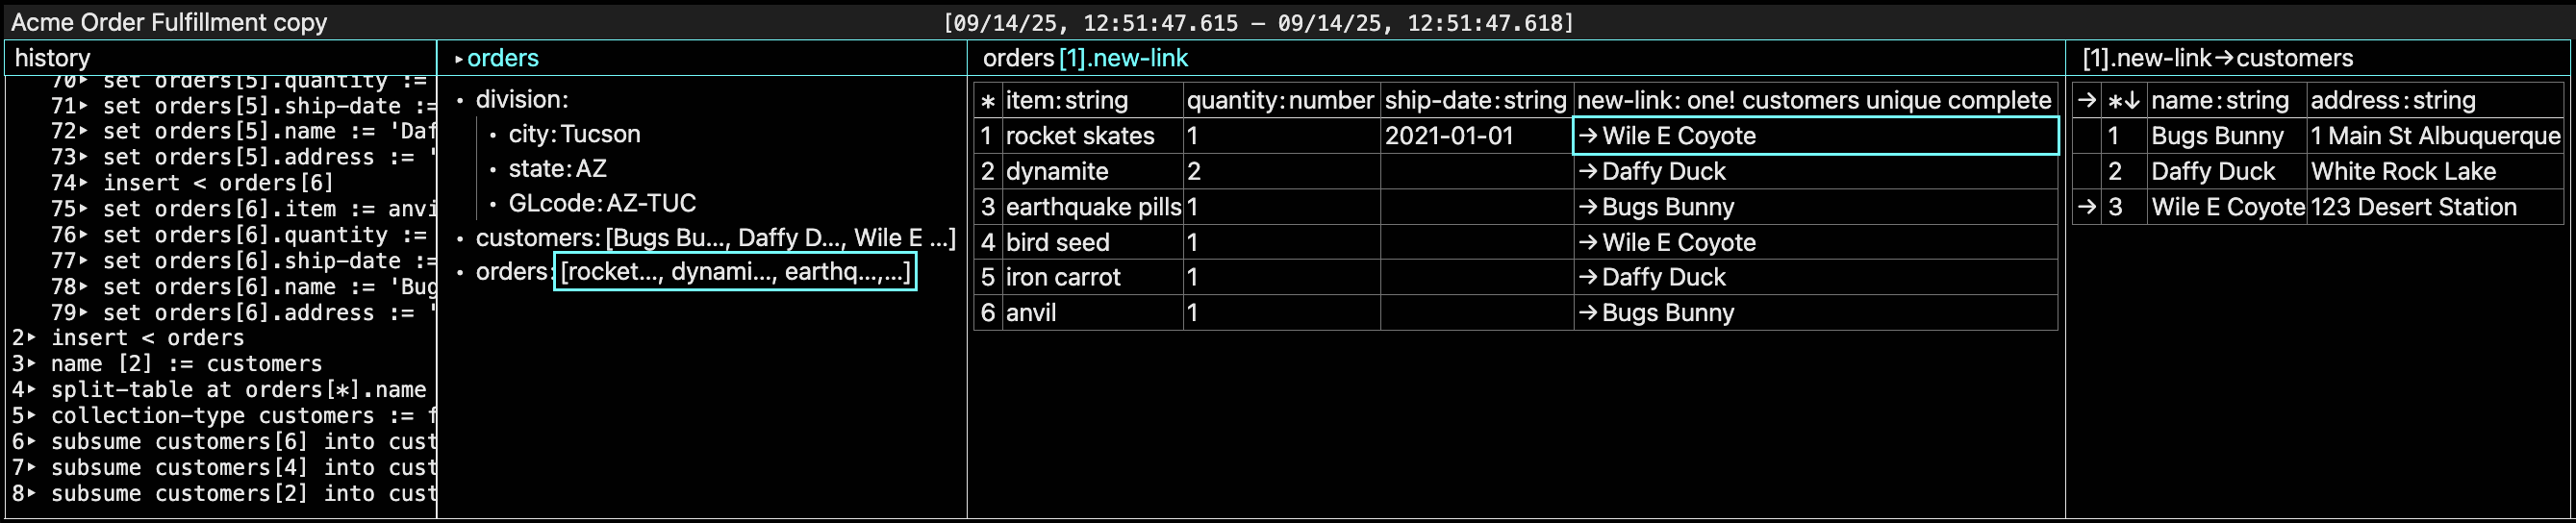
\includegraphics[width=\textwidth]{GUI.png}
\caption{The Baseline UI}
\label{fig:UI-plain}
\end{figure}

Baseline manifests all operations in a direction manipulation UI (Figure~\ref{fig:UI-plain}) that gives users the same power as programs. It is difficult to convey the experience of an interactive interface in a written narrative, so we offer the reader a playable demo at \url{https://thebaseline.dev/Prog26submission/}. The UI and playable demo are discussed in Appendices \ref{UI} and \ref{demo}.

The contributions of this paper are:

\begin{enumerate}

\item We introduce \textit{Operational Differencing} by example in the familiar setting of typed nested lists and records supplied with a rich set of operations
including refactorings. We define the primitive transformations \textit{projection} and \textit{retraction} and the rules governing them.

\item Using these primitives we reconstruct the key features of version control: \textit{diffing} and \textit{transfer} (a specialization of merging more like cherry-picking). Because our technique is operation-based we are able to do fine-grained diffing and merging despite intervening structural transformations.

\item We develop a simplified form of version control without a repo: artifacts under version control have an append-only history of operations attached to them. Branching is just making a copy of the artifact with its history, which can then diverge. There is no need for a repo to record a graph of branches and merges because that can be synthesized from the histories on need, and can be done so optimally in a well-defined sense. By liberating branches and versions of artifacts from the repo they can be shared freely and independently, much like the ubiquitous folk practice of file copying~\cite{Burnett14, Basman19}, but with the added benefit of being able to diff and merge.

\item We enrich the data model to incorporate relational databases, including operations for schema change and normalization. We demonstrate version control on databases that works across schema changes, and which can also be used to manage schema migrations.

\item We conjecture that queries can be \textit{operationalized} into a sequence of schema and data operations, in a form of Programming by Demonstration~\cite{cypher93-pbd}. We develop this idea on a query language fragment containing selects and joins. Operationalized queries are represented as a \textit{future timeline} that is speculatively executed as a branch off of the present state, returning a value from its \textit{hypothetical future}. This conjecture could open up an unexplored space of query language designs.

\item Operationalized queries have a perhaps surprising benefit: query rewriting~\cite{curino08, herrmann17} during schema change falls out ``for free'' from the machinery of operational differencing.

% \item We demonstrate Baseline's direct manipulation UI that supports interactive data and schema changes as well as diffing and merging between databases.
% Miller columns~\cite{miller-columns} are used to drill into nested data and across relationhips, with each column containing an indented outline or a flat table. We discuss our design iteration on visualizing differences in the presence of rich transformations, leading to a split screen with coordinated selection. A \textit{Playable Demo} is available.

\item Altogether we develop solutions to four out of eight challenge problems of schema evolution~\cite{challenge-problems}.

\end{enumerate}

% The superpower of our operation-based approach to schema evolution and version control is that, compared to traditional state-based approaches, it captures user intentions more accurately. We also seek to make these capabilities more concrete and interactive through a direct manipulation UI, reducing as much as we can the need for ad hoc scripting. Throughout, we seek to make things easier though conceptual simplification.
% In summary, the goal of Baseline is to support all the dimensions of data evolution \textit{fluently}---with ease and accuracy.






\section{Rich Data Operations}\label{rich-data}

We start with familiar data structures: nested lists and records. The atomic values are strings, supplied in the set \mathbox{S}, and numbers, supplied in \mathbox{N}, including \mathbox{\textsf{NaN}}. What is unusual about this data model is that we assign permanent unique identifiers (IDs) to every record field and list element. These IDs are supplied from the disjoint sets \mathbox{F} for record fields and \mathbox{E} for list elements. Because record fields have unique IDs their names are only for human readability and we elide them in most examples. Another unusual feature is that deletion of a record field or list element leaves behind a \textit{tombstone} (see Appendix~\ref{deletion}).

% \begin{remark}
%   IDs and tombstones are not essential. They are invisible in the UI and do not affect value equality. We have prototyped an implementation without IDs and our current implementation doesn't use tombstones. They are bookeeping information stored in the state that greatly simplifies the description of the system, which is why we adopt them here. IDs also improve performance.
% \end{remark}

The data model is typed similarly to statically typed Functional Programming (FP) language such as ML, as follows. List elements all have the same type as defined in the type of the list (tombstones are a bottom type). Record values have the same sequence of fields with the same ID and type of value as in the type of the record. The elements of a list and the fields of a record must have different IDs.
%Record fields are named with a string which need not be unique.
The empty record \mathbox{\text{\{\}}}serves as a unit type. Every type has an \textit{initial value}.
We omit sum types and type aliases because they are not needed in this paper.
Figure~\ref{rich-data} defines the syntax and operations of the model.

% data syntax table
\begin{figure}[h]
\tcbox{
  \begin{minipage}{\textwidth}
\[ \begin{array}{r@{\ }l|r@{\ }l|r@{\ }l|l}
  \multicolumn{2}{l|}{\textrm{type}} & \multicolumn{2}{l|}{\textrm{value}} & \multicolumn{2}{l|}{\textrm{initial value}}&\\
  \hline
  T \Coloneqq & & v \Coloneqq & & T^\varnothing = & &\\
  &  \textsf{String} & & S & & \emptystring & \textrm{string}\\
  & \textsf{Number} & &  N & & \textsf{NaN} & \textrm{number}\\
  & \textsf{List } T & & [ E \is v \  \dots ] & & [] & \textrm{list}\\
  %& \{ F \  S \is T \  \dots \} & & \{ F \is v \  \dots \} & & \{ F \is T^\varnothing \  \dots \}& \textrm{record}\\
  & \{ F \  S \is T \  \dots \} & & \{ F \is v \  \dots \} & & \{ F \is T^\varnothing \  \dots \}& \textrm{record}\\

  & \bot && \bigtimes & & \bigtimes & \textrm{tombstone}\\
\end{array}\]

% data operations table
\[
\hspace{-22pt}
\begin{array}{l|l}
  \textrm{Value operations} & \\
  \hline
  p \textsf{ noop} & \textrm{Do nothing}\\
  p \textsf{ write } v & \textrm{Write atomic value $v$ at $p$}\\
  % p \textsf{ init } & \textrm{Set $p$ to initial value}\\

  p \textsf{ insert } E \textsf{ before } E' & \textrm{Insert element ID $E$ into list at $p$ in front of element $E'$}\\
  p \textsf{ append } E & \textrm{Append element ID $E$ to end of list at $p$}\\

  p \textsf{ delete } E & \textrm{Delete element ID $E$ in list at $p$}\\

  p \textsf{ move } p' & \textrm{List element $p$ is copied to $p'$ in same list then $p$ is deleted}\\
  \hline

  \textrm{Type operations} & \rule[0pt]{0pt}{16pt}\\
  \hline
  p \textsf{ Define } T & \textrm{Define $p$ to have type $T$, initializing values}\\
  p \textsf{ Convert } T & \textrm{Convert atomically-typed $p$ to atomic type $T$}\\

  p \textsf{ Rename } S & \textrm{Rename record field $p$ to string $S$}\\

  p \textsf{ Insert } F \textsf{ before } F' & \textrm{Insert field ID $F$ into record at $p$ in front of field $F'$}\\
  p \textsf{ Append } F & \textrm{Append field ID $F$ to end of record at $p$}\\

  p \textsf{ Delete } F & \textrm{Delete field ID $F$ in record at $p$}\\

  p \textsf{ Move } p' & \textrm{Record field at $p$ is copied to $p'$ in the same record}\\
  & \textrm{or containing\slash contained record, and then $p$ is deleted}\\


  p \textsf{ ListOf } & \textrm{Convert value at $p$ into a list of one element with ID $\mathbb{1}$}\\
  p \textsf{ IntoFirst } & \textrm{Convert list at $p$ into its first element, else the initial value} \\

  p \textsf{ RecordOf } F & \textrm{Convert value at $p$ into a record of one field with ID $F$} \\
  p \textsf{ IntoField } F & \textrm{Convert record at $p$ into value of its field $F$} \\

\end{array}\]
\end{minipage}
}
\caption{Rich data syntax and operations}
\label{fig:rich-data}
\end{figure}


A \textit{path} \mathbox{p} is a possibly empty sequence of IDs denoting a path drilling into nested records and lists. Paths can access both values and types. We separate the IDs in a path with dots, and a single dot is the empty (top) path. A special element ID~\mathbox{*} is used to access the element type of a list type.

A \textit{state} pairs a value with its type. We abuse the notation \mathbox{v \isa T} to both denote a state and assert that the value matches the type.
An \textit{operation} is a partial function from an \textit{input state} to an \textit{output state}. Operations are not defined on all input states, imposing various preconditions.
All operations take a \textit{target} path as a parameter indicating that the operation is to be performed at that path within the state.
Operation use infix syntax, placing the target path first, then the operation name, followed by any other parameters.

% For example the \textsf{write} operation takes a value as another parameter and writes that value into the target path. The \textsf{write} operation requires that the target path exists in the value and that its type matches the value parameter.



We execute operations with the \mathbox{\fatsemi} infix operator taking an input state on the left, an operation on the right, and yielding an output state which may be chained into subsequent executions. Here is an example that starts with an empty list of numbers and adds an element with ID $e$ and value $1$:
\begin{align*}
  S_1 &= [] \isa \textsf{List Number}\\
  S_2 &= S_1 \exec \ldotp \textsf{ append } e \exec \ldotp e \textsf{ write } 1\\
  &= [e \is 1] \isa \textsf{List Number}\\
\end{align*}
\vspace{-30pt}\\
The \textsf{append} targets the empty path \mathbox{\ldotp} referring to the whole list. Then the \textsf{write} targets the new element with the path \mathbox{\ldotp e}. In all our examples we take IDs like \mathbox{e} as given but in practice the Baseline API generates them uniquely.

A \textit{table} is a list of records, the fields of which are the \textit{columns} while the elements of the list are the \textit{rows}. Here is an example of changing the type of a table:
\begin{align*}
S_1 &= [e \is \{x \is 1 \comma  y \is 2\}] \isa \textsf{List} \{x \is \textsf{Number}\comma  y \is \textsf{Number}\}\\
S_2 &= S_1 \exec \ldotp * \textsf{ Append } z \exec \ldotp * \ldotp z \textsf{ Define Number}\\
 &= [e \is \{x \is 1\comma  y \is 2,\ z\is \textsf{NaN}\}] \isa \textsf{List} \{x \is \textsf{Number}\comma  y \is \textsf{Number}\comma z\is \textsf{Number}\}\\
\end{align*}
\vspace{-30pt}\\
The \textsf{Append} operation targets the path \mathbox{\ldotp *} which is the record type of the list's elements and adds a new field \mathbox{z} to it, in effect adding a column to the table. The \textsf{Define} operation targets the path \mathbox{\ldotp  * \ldotp z} which is the type of the new field (initially the unit type \mathbox{\{\}}) and changes it to \mathbox{\textsf{Number}}. The new field is also inserted into all elements of the list with the initial value \mathbox{\textsf{NaN}}.

The \textsf{append} and \textsf{write} operations are \textit{value operations}, meaning they do not modify the type of the state. On the other hand \textsf{Append} and \textsf{Define} are \textit{type operatons} that may modify both the type and value. Type operations do \textit{schema migration}: the value is adapted to match the type while minimizing loss of information, iterating over list elements as needed (think of the \mathbox{*} in the type path as a wildcard). By convention we capitalize the name of type operations. Baseline has a \textit{user mode} in which only value operations are permitted.

\begin{remark}
In this presentation we adopt the standard approach of defining values and types as distinct mathematical objects. Actually Baseline only has values, with initial values serving as prototypes. Every list contains an initial \textit{header} element with the ID~\mathbox{*} containing an initial value which serves as the prototype of the list elements. Note how this convention corresponds to the visual rendering of a table where a header row describes the type of each column. Types are a powerful abstraction for the theory and implementation of programming systems but we conjecture that they can be replaced with prototypes, without loss of power, to simplify the programming experience. We have also explored an untyped version of our approach~\cite{denicek}.
\end{remark}

Many of the type operations exist in order to do schema migration on values: they would not be needed just to define a type prior to populating it with data. We think of these operations as \textit{type refactorings}, capturing high-level design changes. They are manifested in the UI as direct manipulations so that schema evolution can be done interactively. Schema evolution is also needed in \textit{live programming}~\cite{challenge-problems}.
\begin{figure}[h]
\begin{align*}
  S_1 &= [
    e \is \{ \mathit{what}\is \quotedstring{clean}\comma  \mathit{who}\is \quotedstring{Jack} \}
    ] \isa
    \textsf{List}\{ \mathit{what}\is \textsf{String}\comma \mathit{who}\is \textsf{String} \}\\
S_2 &= S_1 \exec \ldotp *\ldotp \mathit{who} \textsf{ ListOf } \\
 &= [
    e \is \{ \mathit{what}\is \quotedstring{clean}\comma  \mathit{who}\is [\mathbb{1}\is \quotedstring{Jack}] \}
    ] \isa
    \textsf{List}\{ \mathit{what}\is \textsf{String}\comma  \mathit{who}\is \textsf{List String} \}\\
\end{align*}
\vspace{-40pt}
\caption{TODO refactoring}
\label{fig:TODO-refactor}
\end{figure}

For example a common design evolution is when a single value needs to become a list of multiple values. We capture this in the \textsf{ListOf} operation, shown on a TODO table in Figure~\ref{fig:TODO-refactor}.
The \textsf{ListOf} operation takes any type and wraps it inside a list, and wraps all corresponding values into single-element lists using the element ID $\mathbb{1}$. We will return to this example in the next section.


% \subsection{Much Ado About Nothing}
% Possibly merge with deletion
% Conjecture: don’t need Null, Option, Result
% Snobol and verse show we don't need Results
% Conjecture: common-sense solution to the conundrum of nulls.
% Mention along with sums?
% Or just skip as irrelevant and argument-triggering
% but this is an independent decision
% Exception is numbers, but already have familiar NaN
% Maybe skip initial values?


\section{Operational Differencing}

Change management systems deal with what happens when two copies (or replicas or branches) of something diverge.
These systems split into \textit{state-based} and \textit{operation-based} approaches~\cite{diff3, Shapiro11}.
In this section we introduce a new form of operation-based change management: \textit{Operational Differencing}.

The benefit of operation-based techniques is that they can capture more information than can be inferred from the states.
For example a \textsf{Rename} operation makes many changes throughout the state, and standard version control systems will see these changes as unrelated and conflicting with any other changes on the same text lines. In contrast operational differencing sees a renaming as a single change that conflicts only with renaming to a different name.
The benefit of state-based techniques is that they can observe other systems from the outside, which may explain why all existing version control systems are state-based.

\begin{remark}
We discuss source code version control systems like git~\cite{ProGit} as a point of reference, but we do not propose to compete with them. Git is highly adapted to the needs of intensive development in the Unix environment and the cultural norms of Unix developers. In that context version control must be state-based in order to interoperate with existing tools and practices. Instead of source code we focus on rich data, where we believe operation-based version control offers important benefits.
\end{remark}

We define a \textit{timeline} to be an initial state and a sequence of operations executed in order that are each valid on their input state, producing an end state.
A \textit{history} is a timeline starting from the initial empty state of a document, which by convention is the unit value.
Baseline records histories by observing the operations executed in the API and in a UI that manifests operations as direct manipulations. Operational differencing is built upon two primitive functions on operations: \textsf{Project} and \textsf{Retract}.

\subsection{Projection}

% projection diagrams
\begin{figure}[h]
\begin{minipage}[b][][b]{1.75in}
\center
\begin{tikzcd}[column sep=large]
	0 & {[\mathbb{1}\is 0]} \\
	2 & {[\mathbb{1}\is 2]}
	\arrow["{{\ldotp \textsf{ ListOf}}}", from=1-1, to=1-2]
	\arrow["{{\ldotp \textsf{ write } 2}}"'{pos=0.4}, from=1-1, to=2-1]
	\arrow["{{\textsf{P}\Rightarrow}}"{description, pos=0.2}, draw=none, from=1-1, to=2-2]
	\arrow["{{\ldotp\mathbb{1} \textsf{ write } 2}}"{pos=0.4}, dashed, from=1-2, to=2-2]
	\arrow["{{\ldotp \textsf{ ListOf}}}"', dashed, from=2-1, to=2-2]
\end{tikzcd}
\\[4pt]
(a)
\end{minipage}
\quad
\begin{minipage}[b][][b]{1.75in}
\center
\begin{tikzcd}[column sep=large]
	0 & 1 \\
	2 & 2
	\arrow["{{\ldotp \textsf{ write } 1}}", from=1-1, to=1-2]
	\arrow["{{\ldotp \textsf{ write } 2}}"'{pos=0.4}, from=1-1, to=2-1]
	\arrow["{{\textsf{P}\Rightarrow}}"{description, pos=0.2}, draw=none, from=1-1, to=2-2]
	\arrow["{{\ldotp \textsf{ write } 2}}"{pos=0.4}, dashed, from=1-2, to=2-2]
	\arrow["{{\ldotp \textsf{ noop}}}"', dashed, from=2-1, to=2-2]
\end{tikzcd}
\\[4pt]
(b)
\end{minipage}
\quad
\begin{minipage}[b][][b]{1.25in}
\center
\begin{tikzcd}[column sep=large]
	\bullet & \bullet \\
	\bullet & \bullet
	\arrow["{\mathit{base}}", from=1-1, to=1-2]
	\arrow["{\mathit{pre}}"'{pos=0.4}, from=1-1, to=2-1]
	\arrow["{\textsf{P}\Rightarrow}"{description, pos=0.2}, draw=none, from=1-1, to=2-2]
	\arrow["{\mathit{post}}"{pos=0.4}, dashed, from=1-2, to=2-2]
	\arrow["{\mathit{adjust}}"', dashed, from=2-1, to=2-2]
\end{tikzcd}
\\[4pt]
(c)
\end{minipage}
\caption{Projection}
\label{fig:projection}
\end{figure}

The \textsf{Project} function takes as inputs two timelines with the same initial state and produces two new timelines continuing from the input timelines and converging on the same final state. It is easier to understand this with diagrams.
In Figure~\ref{fig:projection}(a) the arrow on the left takes the state \mathbox{0} (we elide the obvious type signature) and writes a \mathbox{2} over it. The arrow on the top wraps that \mathbox{0} into a list with one element \mathbox{[\mathbb{1}\is 0]}. The projection function takes these two arrows as input and produces the two dashed arrows such that the diagram \textit{commutes}, meaning the dashed arrow operations are valid on the states at their bases, and they both produce the same state \mathbox{[\mathbb{1}\is 2]}. The way this is achieved is to map the target path of the \textsf{write} operation through the \textsf{ListOf} operation producing the operation \mathbox{\ldotp\mathbb{1} \textsf{ write } 2}. We say that the two \textsf{write} operations have the same \textit{intention}---they ``do the same thing'' in different states---they convert the \mathbox{0} to a \mathbox{2}, even though the \mathbox{0} has moved to a different location. That is the key principle of projection: it produce a right-hand operation that ``does the same thing'' as the left-hand operation despite the top operation having intervened.

Figure~\ref{fig:projection}(b) shows a messier situation. Here the left and top operations are both writing different values to the same location. This is called a \textit{conflict}. The rule is that projection attempts to preserve the intention of the left operation, even if that means overriding the top operation, which as a consequence gets converted to a \textsf{noop} on the bottom.

This last example shows that projection is asymmetric: flipping the diagram on its diagonal to switch left and top yields a different result. And in fact we will have occasion to flip and rotate these diagrams, so we cannot depend on terminology like ``left'' and ``top''. Figure~\ref{fig:projection}(c) shows our orientation-neutral terminology: projection converts the \textit{pre} operation into the \textit{post} operation, preserving its intent after the \textit{base} operation intervenes. The \textit{base} operation is converted into the \textit{adjust} operation preserving as much of its intention as is allowed by the first rule. We also graphically indicate the orientation of the diagram by placing \mathbox{\textsf{P}\!\Rightarrow} into the corner of the initial state.


% projection rules
\begin{figure}[h]
\begin{minipage}[b][][b]{1.6in}
\center
\begin{tikzcd}[column sep=large]
	\bullet & \bullet \\
	\bullet & \bullet
	\arrow["{{p \textsf{ ListOf}}}", from=1-1, to=1-2]
	\arrow["{{p \ldotp\ldotp q  \ A}}"'{pos=0.4}, from=1-1, to=2-1]
	\arrow["{{\textsf{P}\Rightarrow}}"{description, pos=0.2}, draw=none, from=1-1, to=2-2]
	\arrow["{{p \ldotp \mathbb{1} \ldotp\ldotp q \ A}}"{pos=0.4}, dashed, from=1-2, to=2-2]
	\arrow["{{p \textsf{ ListOf}}}"', dashed, from=2-1, to=2-2]
\end{tikzcd}
\\[4pt]
(a)
\end{minipage}
\quad
\begin{minipage}[b][][b]{1.7in}
\center
\begin{tikzcd}[column sep=large]
	\bullet & \bullet \\
	\bullet & \bullet
	\arrow["{{p \textsf{ write } w}}", from=1-1, to=1-2]
	\arrow["{{p \textsf{ write } v}}"'{pos=0.4}, from=1-1, to=2-1]
	\arrow["{{\textsf{P}\Rightarrow}}"{description, pos=0.2}, draw=none, from=1-1, to=2-2]
	\arrow["{{p \textsf{ write } v}}"{pos=0.4}, dashed, from=1-2, to=2-2]
	\arrow["{{p \textsf{ noop}}}"', dashed, from=2-1, to=2-2]
\end{tikzcd}
\\[4pt]
(b)
\end{minipage}
% \quad
% \begin{minipage}[b][][b]{1.6in}
% \center
% \begin{tikzcd}[column sep=large]
% 	\bullet & \bullet \\
% 	\bullet & \bullet
% 	\arrow["{{p \ A}}", from=1-1, to=1-2]
% 	\arrow["{{p \ A}}"'{pos=0.4}, from=1-1, to=2-1]
% 	\arrow["{{\textsf{P}\Rightarrow}}"{description, pos=0.2}, draw=none, from=1-1, to=2-2]
% 	\arrow["{{p \textsf{ noop}}}"{pos=0.4}, dashed, from=1-2, to=2-2]
% 	\arrow["{{p \textsf{ noop}}}"', dashed, from=2-1, to=2-2]
% \end{tikzcd}
% \\[4pt]
% (c)
% \end{minipage}
\caption{Projection rules}
\label{fig:projection-rules}
\end{figure}

Projection is defined with rules that can be diagrammed similarly. Figure~\ref{fig:projection-rules}(a) is a rule covering the \textsf{ListOf} example. The target path of the \textsf{ListOf} is abstracted to \mathbox{p}, and the \textsf{write} operation is abstracted into any operation \mathbox{A} targeting \mathbox{p} or deeper, which is indicated with the path concatenation operator in \mathbox{p \ldotp\ldotp q}. Operation \mathbox{A} is projected down into the \textsf{ListOf} with the path \mathbox{p \ldotp \mathbb{1} \ldotp\ldotp q}.

Figure~\ref{fig:projection-rules}(b) is the rule for conflicting writes.
% Figure~\ref{fig:projection-rules}(c) is a generic rule that identical operations cancel out in projection, which overrides all the other rules. HoW?


\subsection{Retraction}

% retraction diagrams
\begin{figure}[h]
\begin{minipage}[b][][b]{1.2in}
\center
\begin{tikzcd}[column sep=large]
	\bullet & \bullet \\
	\bullet & \bullet
	\arrow["{{\mathit{base}}}", from=1-1, to=1-2]
	\arrow["{{\mathit{pre}}}"'{pos=0.4}, dashed, from=1-1, to=2-1]
	\arrow["{{\Leftarrow\textsf{R}}}"{description, pos=0.2}, draw=none, from=1-2, to=2-1]
	\arrow["{{\mathit{post}}}"{pos=0.4}, from=1-2, to=2-2]
	\arrow["{{\mathit{adjust}}}"', dashed, from=2-1, to=2-2]
\end{tikzcd}
\\[4pt]
(a)
\end{minipage}
\quad
\begin{minipage}[b][][b]{1.8in}
\center
\begin{tikzcd}[column sep=large]
	0 & {[\mathbb{1}\is 0]} \\
	2 & {[\mathbb{1}\is 2]}
	\arrow["{{\ldotp \textsf{ ListOf}}}", from=1-1, to=1-2]
	\arrow["{{\ldotp \textsf{ write } 2}}"'{pos=0.4}, dashed, from=1-1, to=2-1]
	\arrow["{{\Leftarrow\textsf{R}}}"{description, pos=0.2}, draw=none, from=1-2, to=2-1]
	\arrow["{{\ldotp\mathbb{1} \textsf{ write } 2}}"{pos=0.4}, from=1-2, to=2-2]
	\arrow["{{\ldotp \textsf{ ListOf}}}"', dashed, from=2-1, to=2-2]
\end{tikzcd}
\\[4pt]
(b)
\end{minipage}
\quad
\begin{minipage}[b][][b]{1.75in}
\center
\begin{tikzcd}
	0 & {[\mathbb{1}\is 0]} \\
	{} & {[\mathbb{1}\is 2\comma e \is \textsf{NaN}]}
	\arrow["{{\ldotp \textsf{ ListOf}}}", from=1-1, to=1-2]
	% \arrow["{{}}"'{pos=0.4}, dashed, "/" marking, from=1-1, to=2-1]
	\arrow["{{\nLeftarrow\textsf{R}}}"{description, pos=0.2}, draw=none, from=1-2, to=2-1]
	\arrow["{{\ldotp \textsf{ append } e}}"{pos=0.4}, from=1-2, to=2-2]
	% \arrow["{{}}"', dashed, "/" marking, from=2-1, to=2-2]
\end{tikzcd}
\\[4pt]
(c)
\end{minipage}
\caption{Retraction}
\label{fig:retraction}
\end{figure}

The \textsf{Retract} function goes in the opposite direction of \textsf{Project}. Figure~\ref{fig:retraction}(a) shows that it starts with two timelines \textit{base} and \textit{post} and produces \textit{pre} and \textit{adjust}. We say that \textit{post} is retracted through \textit{base} into \textit{pre}. The goal as with projection is that \textit{pre} preserves the intention of \textit{post} before \textit{base} happened---it ``does the same thing''. Likewise \textit{adjust} preserves the intention of \textit{base} but defers to the first rule.

Figure~\ref{fig:retraction}(b) shows the retraction reversing the projection in Figure~\ref{fig:projection}(a). Often retraction is the inverse of projection as in this case, but not always, and sometimes retraction is not possible at all. In Figure~\ref{fig:retraction}(c) the list has a new element appended to it. There is no way to do the same thing before the list was created. Projection failures indicates a \textit{dependency} between operations. The \textsf{append} operation depends on the prior \textsf{ListOf} operation having created the list and cannot be retracted through it.

Retraction is defined with rules like those for projection so we skip over them in the interest of brevity.
\begin{note}
  Baseline implements projection and retraction rules with procedural if and switch statements, which has become unwieldy as the number of operations has grown, so much so that the implementation is incomplete. It should be possible to define a declarative DSL that exploits the inherent symmetries in the rules: projection is often symmetric in the two input operations; projection and retraction are often inverses. See \S~\ref{discussion}.
\end{note}

\begin{remark}
How do we know if the rules for projection and retraction are correct, that they do indeed preserve the intentions of operations? Our answer is that there is no objective answer to this question. The rules are essentially axioms defining what it means to preserve intention. Well-designed rules will agree with intuition and avoid surprises. One of these intuitions is that transfer should be symmetric: transfering an operation across a diff and then transferring it back again should bring back the same operation (or in some cases grounding out into a \textsf{noop}). We call this the \textit{roundtrip law} and we test that our rules obey it.
% Except there are exceptions, like when an operation gets dropped because its target was deleted. The law has weakened as we discovered these exceptions, so in future work we hope to establish a more principled basis.


% % note have dropped the override rule because it is awkward to explain
% % note duplication in a join probably breaks this principle! But that only comes later
% % correctness -> laws
% Nevertheless there are some principles we can expect any system of transfer rules to follow. One of them is that projection and retraction should be inverses---that transferring an operation to a different branch and then back again should return it unchanged. After all ``doing the same thing'' seems like a symmetric relation. Unfortunately we have aleady seen examples where an operation gets wiped out during transfer into a \textsf{noop}, which will always return as a \textsf{noop}. Therefore we weaken the principle to say that roundtripping an operation must return an operation that does the same thing or less than the original. To make that precise we define an ordering on branches \mathbox{\leq}:
% \[
% O; a \leq O; b \quad\textrm{iff} \quad
% \begin{tikzcd}
% 	O & B \\
% 	A & B
% 	\arrow["{b}", from=1-1, to=1-2]
% 	\arrow["{a}"'{pos=0.4}, from=1-1, to=2-1]
% 	\arrow["{\textsf{P}\Rightarrow}"{description, pos=0.2}, draw=none, from=1-1, to=2-2]
% 	\arrow[dashed, from=1-2, to=2-2]
% 	\arrow[dashed, from=2-1, to=2-2]
% \end{tikzcd}
% \]
% in other words, projecting $a$ through $b$ makes no difference. The \textbf{Roundtrip Monotonicity} principle asserts that (a) \mathbox{\leq} is a partial order, and (b) roundtripping a timeline through a projection and retraction or the reverse will result in a timeline $\leq$ the original.

% We also need to prove that diffs are indeed optimal.
\end{remark}

\subsection{Across the Multiverse}\label{transfer}

  A \textit{diff} between two states \mathbox{A} and \mathbox{B} is a pair of timelines that branch off some shared state \mathbox{O} resulting in \mathbox{A} and \mathbox{B}, diagrammed like this:
\[\begin{tikzcd}
	A & {} & {} & O & {} & {} & B
	\arrow["{{a_n}}"', from=1-2, to=1-1]
	\arrow[dotted, from=1-3, to=1-2]
	\arrow["{{a_1}}"', from=1-4, to=1-3]
	\arrow["{b_1}", from=1-4, to=1-5]
	\arrow[dotted, from=1-5, to=1-6]
	\arrow["{b_m}", from=1-6, to=1-7]
\end{tikzcd}\]

The two timelines are called the \textit{branches} of the diff and we call their operations the \textit{differences}. Many version control systems use something like a diff by looking for the \textit{last common ancestor} in a tree of branching versions, which is then used for \textit{three-way diffing}~\cite{diff3}. We do not do that---we will discuss how to calculate a diff in \S\ref{diff-synth} but for the moment let us take them as given. The key operation on a diff is to
\textit{transfer} an operation from one side to another, which we define diagrammatically in Figure~\ref{fig:transfer} (where we lift projection and retraction from operations to timelines in the obvious way).
\vspace{-16pt}
\begin{figure}[h]
\[
\textsf{Transfer}(a_{1\ldots n}, O, b_{1\ldots m}) = b' \textrm{ in }\quad
\begin{tikzcd}[column sep = huge]
	A_{n-1} & O & B \\
	A_n & {O'} & {B'}
	\arrow["{a_n}"', from=1-1, to=2-1]
	\arrow["{\textsf{R}\Rightarrow}"{description, pos=0.1}, draw=none, from=1-1, to=2-2]
	\arrow["{a_{n-1}\,\ldots\  a_1}"', from=1-2, to=1-1]
	\arrow["{b_1\,\ldots \  b_m}", from=1-2, to=1-3]
	\arrow["o", dashed, from=1-2, to=2-2]
	\arrow["{\textsf{P}\Rightarrow}"{description, pos=0.2}, draw=none, from=1-2, to=2-3]
	\arrow["{b'}", dashed, from=1-3, to=2-3]
	\arrow["{\mathit{adjust}_a}"', dashed, from=2-2, to=2-1]
	\arrow["{\mathit{adjust}_b}", dashed, from=2-2, to=2-3]
\end{tikzcd}\]
\vspace{-16pt}
\caption{Transfer}
\label{fig:transfer}
\end{figure}

Transfer\footnote{Transfer was called migrate in earlier publications~\cite{edwards21, edwards22}.} retracts \mathbox{a_n} backwards through all earlier operations on the \mathbox{A} timeline onto the original state \mathbox{O} and then projects that operation forwards through all the operations of the \mathbox{B} timeline. The final result is the operation \mathbox{b'} that yields a new version \mathbox{B'}. The effect of the transfer is that the final operation \mathbox{b'} preserves the intention of the original operation \mathbox{a_n} given all the operations traversed while traveling backward in time to \mathbox{O} and then forward to \mathbox{B}. Transfer also computes a new diff between \mathbox{A_n} and \mathbox{B'}: the transferred operation is now shared between them in \mathbox{O'} with branching timelines \mathbox{\mathit{adjust}_a} and \mathbox{\mathit{adjust}_b}. This updated diff is used later for diff optimization (\S\ref{diff-synth}).

In this definition we transferred the last operation of the \mathbox{A} branch---an earlier operation can be transferred by using the corresponding truncation of \mathbox{A}.
Since transfer uses retraction it may fail because of a dependency on an earlier operation in the \mathbox{A} branch. However it is always possible to transfer any operation by first transfering all of its dependencies earlier in the branch. A \textit{sync} action that transfers all operations in the branch will always succeed. We also provide a finer-grained \textit{dependency transfer} function that transfers just the transitive dependencies and so always succeeds.

As an example we extend the TODO refactoring in Figure~\ref{fig:TODO-refactor} into two branches: branch \mathbox{A} reassigns the TODO from Jack to Jill; branch \mathbox{B} converts the assignment into a list, changes the assignment from Jack to Jacque and inserts a new assignment to Tom:
\begin{align*}
  O &= [
    e \is \{ \mathit{what}\is \quotedstring{clean}\comma  \mathit{who}\is \quotedstring{Jack} \}
    ] \\
  % a_1 &= \ldotp e\ldotp\mathit{what}\textsf{ write } \quotedstring{tidy}\\
  a_1 &= \ \ldotp e\ldotp\mathit{who}\textsf{ write } \quotedstring{Jill}\\
  A &= [
    e \is \{ \mathit{what}\is \quotedstring{clean}\comma  \mathit{who}\is \quotedstring{Jill} \}
    ] \\
  b_1 &= \ \ldotp *\ldotp \mathit{who} \textsf{ ListOf } \\
  % b_2 &= \ldotp e\ldotp\mathit{who}\ldotp\mathbb{1} \textsf{ write } \quotedstring{Tom}\\
  b_2 &= \ \ldotp e\ldotp\mathit{who}\ldotp\mathbb{1} \textsf{ write } \quotedstring{Jacque} \\
  b_3 &= \ \ldotp e\ldotp\mathit{who} \textsf{ insert } g \textsf{ before } \mathbb{1} \exec \ldotp e\ldotp\mathit{who}\ldotp g \textsf{ write } \quotedstring{Tom} \\
  B &= [
    e \is \{ \mathit{what}\is \quotedstring{clean}\comma  \mathit{who}\is
    [ g \is \quotedstring{Tom} \comma \mathbb{1}\is \quotedstring{Jacque}] \}
    ] \\
  \end{align*}
  \vspace{-30pt}\\
We can transfer these operations individually from one side to the other.
If we transfer \mathbox{b_2} into \mathbox{A} the change from Jack to Jacque gets applied to the \textsf{who} field (showing the change in bold):
\[A' = [e \is \{ \mathit{what}\is \quotedstring{clean}\comma  \mathit{who}\is \textbf{\quotedstring{Jacque}} \}]\]
If we transfer \mathbox{a_1} into \mathbox{B} the change from Jack to Jill gets applied to the list element containing Jack, even though it has been wrapped and shifted:\\
\[B' = [
    e \is \{ \mathit{what}\is \quotedstring{clean}\comma  \mathit{who}\is
    [ g \is \quotedstring{Tom} \comma \mathbb{1}\is \textbf{\quotedstring{Jill}}] \}
]\]

% diagram one of these examples?

This example demonstrates how transference can propagate changes bidirectionally through structural changes. Standard state-based version control techniques would see only a big conflict and require a human to pick out and propagate finer-grained changes correctly.
Operational differencing does this more precisely because it tracks how locations shift through time.

Version control systems like git provide a variety of actions like \textit{merge}, \textit{rebase}, and \textit{cherry-pick} with subtly different effects. We provide transferrance as the sole primitive and then build coarser-grained actions out of sets of transfers. For example all the changes in one branch can be transferred to the other. Just the type changes or just the data changes can be transferred. The dependency transfer action mentioned earlier transfers all transitive dependencies. To \textit{synchronize} two branches all changes are transferred from one to the other and then all changes remaining in the other branch are transferred back. Note that synchronization has a direction: syncing from \mathbox{A} into \mathbox{B} resolves all conflicts in favor of \mathbox{A}.


\subsection{Diff Optimization and Synthesis}\label{diff-synth}

We have been discussing transference assuming we are given a diff that specifies a shared state and timelines branching off of it. The intuition is that the shared state should contain everything the two final states have in common, and the branches should be just the differences. Not all branching timelines will satisfy that intuition. There might be redundant operations duplicated in both branches, either by coincidence or by explicit transfers. There could also be redundant changes within a branch that override earlier ones. All of these sorts of redundancies are undesirable because they add noise to a visualization of differences, and in some cases can cause transfer to produce surprising results. There is a simple algorithm that can be used to produce optimal diffs using transference itself.

Note that in Figure~\ref{fig:transfer} the bottom of the diagram produces a new diff: two new timelines \mathbox{\mathit{adjust}_a} and \mathbox{\mathit{adjust}_b} branching from a new shared state \mathbox{O'}. These \textit{adjusted} timelines eliminate the redundancy of the original operation and its transferred image. Clearly after executing a transfer we should drop the original diff and use the adjusted diff instead. In the same way we can use transfers to remove redundancies in diffs as follows. Given a pair of branching timelines we iterate over all the actions on both sides in order\footnote{The order in which the two branches are interleaved does not matter because of the roundtrip law.}. For each operation we try to transfer it to the other branch. If the transfer succeeds and is a fixpoint (it doesn't alter the state of the other side), then we discard the branches in favor of the adjusted ones and continue the loop. The intuition here is that if the transferred operation makes no difference to the other side then it isn't really a difference, so we append it to the history of the shared state. After we have tried every transfer from both sides the result will be optimal in the sense that the history of the shared state is maximal while the timelines branching off of it are minimal, without redundancies. Note however that this maximal shared state may not have ever actually occurred in either history---it is the \textit{hypothetical} ideal last common ancestor if history had happened in a fortuitously non redundant order. This ideal common ancestor avoids the problems that can be caused by cherry-picking in git~\cite{philomatics-git}.

Diff optimization lets us synthesize an optimal diff from the histories of any two states. A history always starts from the unit value as its initial state. So all histories are branches from the initial state and we just optimize that primordial diff.

\begin{note}
  We left out a detail in the diffing algorithm. Sometimes changes cancel each other out, like an insert followed later by a delete, or an operation followed later by its \textit{undo} (Appendix~\ref{undo}). The diff timelines are simplified by attempting to fully retract each operation---if the retraction results in a \textsf{noop} it was canceled out and the simplified adjusted timeline is used instead.
\end{note}

\subsection{Low-fuss Version Control}

The ability to synthesize diffs for any two histories avoids the need for a \textit{repo} to determine the last common ancestor for operations like merging. As we have seen that can be sub-optimal as a basis for three-way diffing. But more importantly, understanding and maintaining the repo imposes a large mental burden on the users of version control systems. Git is infamous for causing confusion and frustration~\cite{perez13, church2014case, xkcd1597}.

We present the user with a simpler conceptual model: every document has an append-only history. To branch an alternate version of a document, simply copy it. The copies can then diverge, and their histories can be compared at any time to compute their diff, which can then be used to transfer differences between them. We can record copy and transfer events as comments in histories in order to reconstruct a version graph like that maintained in a repo.

This approach is more flexible: since versions and branches no longer belong to a repo they can be shared without sharing the whole repo. They are like files (and likely implemented as files): independent storage units that can participate in overlapping and shifting webs of collaboration. They can be emailed. We regain the flexibility of the ubiquitous folk practice of file copying~\cite{Burnett14, Basman19}, but with the added benefit of being able to diff and merge.

\begin{remark}
  Large projects will still need to maintain a list of all branches, but that could be as lightweight as a file directory. Large projects will also want to compress storage and cache diffs. We believe all these capabilities could be added on top of our approach with far less user-facing complexity than git. But that is not an immediate goal: first we want to optimize for small-scale ad hoc usage.
\end{remark}





\section{Database Evolution}\label{db-evolution}
% \section{Relationships}
% \section{Relational Databases}

\begin{figure}
\begin{subfigure}[b]{35em}\vspace{0pt}
  \sffamily
  \small
  \begin{tabular}{ r|l|r|r|l|l|}
  \multicolumn{2}{l}{orders:}\\
     \hhline{~-----}
     ID & item & quantity & ship\_date & name & address \\
     \hhline{~=====}

     $e_1$ & Anvil & 1 & 2/3/23 & Wile E Coyote & 123 Desert Station \\
     \hhline{~-----}
     $e_2$ & Dynamite & 2 & & Daffy Duck & White Rock Lake \\
     \hhline{~-----}
     $e_3$ & Bird Seed & 1 & & Wile E Coyote & 123 Desert Station \\
     \hhline{~-----}
  \end{tabular}
  \caption{Single orders table}
  \label{fig:tables-single}
\end{subfigure}
\\[-0.5em]~\\
\begin{subfigure}[b]{40em}\vspace{0pt}
  \sffamily
  \small
  \begin{tabular}{ r|l|r|r|r|cr|l|l|}
  \multicolumn{2}{l}{orders:}&\multicolumn{4}{l}{}&\multicolumn{2}{l}{customers:}\\
     \hhline{~----~~--}
     ID & item & quantity & ship\_date & customer && ID & name & address \\
     \hhline{~====~~==}

     $e_1$ & Anvil & 1 & 2/3/23 & $\rightarrow\!e_1$ && $e_1$ & Wile E Coyote & 123 Desert Station \\
     \hhline{~----~~--}
     $e_2$ & Dynamite & 2 & & $\rightarrow\!e_2$ && $e_2$ & Daffy Duck & White Rock Lake \\
     \hhline{~----~~--}
     $e_3$ & Bird Seed & 1 & & $\rightarrow\!e_3$ && $e_3$ & Wile E Coyote & 123 Desert Station \\
     \hhline{~----~~--}
  \end{tabular}
  \caption{Split orders and customers tables}
  \label{fig:tables-split}
\end{subfigure}
\\[-0.5em]~\\
\begin{subfigure}[b]{40em}\vspace{0pt}
  \sffamily
  \small
  \begin{tabular}{ r|l|r|r|r|cr|l|l|}
  \multicolumn{2}{l}{orders:}&\multicolumn{4}{l}{}&\multicolumn{2}{l}{customers:}\\
     \hhline{~----~~--}
     ID & item & quantity & ship\_date & customer && ID & name & address \\
     \hhline{~====~~==}

     $e_1$ & Anvil & 1 & 2/3/23 & $\rightarrow\!e_1$ && $e_1$ & Wile E Coyote & 123 Desert Station \\
     \hhline{~----~~--}
     $e_2$ & Dynamite & 2 & & $\rightarrow\!e_2$ && $e_2$ & Daffy Duck & White Rock Lake \\
     \hhline{~----~~--}
     $e_3$ & Bird Seed & 1 & & $\rightarrow\!e_1$ && \multicolumn{3}{l}{}$e_3$\\
     \hhline{~----~~~~}
  \end{tabular}
  \caption{Deduped customers}
  \label{fig:tables-dedup}
\end{subfigure}
\caption{Table schema change}
\label{fig:tables}
\end{figure}

% database syntax and operations
\begin{figure}
\tcbox{
  \begin{minipage}{\textwidth}
\[\begin{array}{r@{\ }l|r@{\ }l|r@{\ }l|l}
  \multicolumn{2}{l|}{\textrm{type}} & \multicolumn{2}{l|}{\textrm{value}} & \multicolumn{2}{l|}{\textrm{initial value}}&\\
  \hline

  & \rightarrow\! p & & \rightarrow\! E & & \rightarrow\! *
  & \textrm{link to element $E$ of list $p$ ($*$ is null link)}  \\

  % multi-link
  % & \rightarrow\! p & & \rightarrow\! [ E \  \dots ] & & \rightarrow\! []
  % & \textrm{link into list } p \\
\end{array}\]
\vspace{.5em}
\[\begin{array}{l|l}
  \textrm{Value operations} & \\
  \hline

  p \textsf{ link } E & \textrm{Link to element } E \textsf{ (unlink if $*$)} \\

  % multi-link
  % p \textsf{ link } E & \textrm{Link to element } E \\
  % p \textsf{ unlink } E & \textrm{Unlink from element } E \\
  \hline

  \textrm{Type operations} & \rule[0pt]{0pt}{16pt}\\
  \hline

  p \textsf{ Link } p' & \textrm{Define $p$ as link to list $p'$} \\

  p \textsf{ Split } p' & \textrm{Split at column $p$ creating linked table $p'$}\\
  p \textsf{ Join } & \textrm{Join link column $p$ deleteing linked table}\\

\end{array}\]
\end{minipage}
}
  \caption{Additional database syntax and operations}
  \label{fig:db-addons}
\end{figure}

In this section we apply Operational Differencing to the problem of \textit{schema evolution} in relational databases. We do this by adding relational database features into our data types and operations.
% We use as a running example \textit{Extract Entity} from~\citet{challenge-problems}.
For example Figure~\ref{fig:tables-single} shows a table of orders for the Acme Corporation. A database professional will immediately see a problem: the customer name and address is duplicated across all orders by the same customer, so any changes to that information would need to be duplicated.
Database textbooks teach to avoid this sort of problem by properly \textit{normalizing} the schema before adding any data. However in practice the need for schema changes often arises after there is data, which must then be \textit{migrated} into the changed schema, typically with ad hoc SQL programs.

One approach a SQL migration program could take is to populate a new \textsf{customers} table from a query projecting out the \textsf{name} and \textsf{address} columns and excluding duplicates. Then it would need to generate primary keys for the deduped customers (the name cannot be the primary key because it is mutable). A new column \textsf{customer} would be added to \textsf{orders} declared as a foreign key containing the customer's primary key. Finally the \textsf{name} and \textsf{address} columns in the \textsf{orders} table would be dropped.

To perform the migration in Baseline we first need to add support for relational data into our types and operations.
We already support tables: they are lists of records, where the elements of the list are the rows and the fields of the record are the columns, which are homogeneously typed as in a relational database.
Throughout the rest of the paper we will refer to any Baseline document containing tables as a \textit{database}.
What is missing so far is \textit{relationships} between tables, which relational databases model through primary and foreign keys. We take a more PL-oriented approach.
Instead of primary keys exposed as user data fields we annotate list elements with IDs that are unique, permanent, and opaque. Instead of foreign keys we add the \textit{link} data type in Figure~\ref{fig:db-addons}: the type of a link defines the table (or list) it ranges over; the value of a link is an element ID in that range, or \mathbox{*} for a null link. We also add the operations defined in Figure~\ref{fig:db-addons}. All operations that move a list must also adjust the path in the type of all links into that list.

The first step in evolving the Acme database is to \textsf{Split} out a \textsf{Customers} table with the following operations:
\[
\begin{array}{ll}
\{ \textsf{orders}\is [ \ldots ]\} \exec & \textrm{(1)}\\
\ldotp \textsf{ Append } \textsf{customers} \exec  & \textrm{(2)}\\
\ldotp \textsf{orders}\ldotp * \ldotp \textsf{name Split customers} \exec & \textrm{(3)}\\
\ldotp \textsf{orders}\ldotp * \ldotp \textsf{name Rename } \quotedstring{customer} & \textrm{(4)}\\
\end{array}\]

% \begin{lstlisting}[mathescape]
% $  \{ \textsf{orders}\is [ \ldots ]\} \exec$
% $\ldotp \textsf{ Append } \textsf{customers} \exec$
% $\ldotp \textsf{orders}\ldotp * \ldotp \textsf{name Split customers} \exec$
% $\ldotp \textsf{orders}\ldotp * \ldotp \textsf{name Rename } \quotedstring{customer}$
% \end{lstlisting}

(1) Starting from the state in Figure~\ref{fig:tables-single};
(2) The \textsf{Append} operation adds a \textsf{customers} field to hold the new table. (3) The \textsf{Split} operation then splits the \textsf{orders} tables in two starting at the \textsf{name} column, copying those columns into the \textsf{customers} table, the rows of which are given the same IDs as in the \textsf{orders} table.
The original \textsf{name} column in \textsf{orders} is replaced with links to the corresponding \textsf{customers} rows.
(4) The \textsf{Rename} operation renames the links column to be \textsf{customer}\footnote{Abusing notation by conflating the name and ID}.
The result is shown in Figure~\ref{fig:tables-split}.

The last step of this database evolution is to de-duplicate the customers, for which we use the \textsf{move} operation from Figure~\ref{fig:rich-data}. Thus:
\[
\ldotp \textsf{customers}\ldotp e_3 \textsf{ move } \ldotp \textsf{customers}\ldotp e_1
\]
The \textsf{move} operation merges \mathbox{e_3} into \mathbox{e_1}, resulting in the state shown in  Figure~\ref{fig:tables-dedup}. Note that the order for Bird Seed has had its link to \mathbox{e_3} forwarded to \mathbox{e_1}. This completes the schema evolution.

\begin{note}
The preceding discussion does not reflect the full complexity of our data model. Lists and tables can be nested. Links are set-valued, and can drill into nested tables. We believe this complexity is justified to cleanly unify PL and DB data models. The \textsf{Split} and \textsf{Join} operations are composed from a set of primitive operations on nested tables and links. We have experimented with several alternative sets of primitives, with subtle tradeoffs on transfer semantics, for example how does appending a column get projected through the split operation? See \S~\ref{discussion}.
\end{note}


% \begin{remark}
%   The \textit{Impedance Mismatch Problem}~\cite{Chen1996} is the fact that PLs and DBs use very different data models, requiring a lot of ad hoc code to translate between them. In our experience it is a large source of inessential complexity in application software. The Baseline project wants to avoid this problem by developing a data model coherently unifying the needs of both PLs and DBs. However that goal is tangential to the subject of this paper so we have included the bare minimum. We believe a fuller unified model should additionally include:
%   \begin{itemize}
%     \item Sum types and type references.
%     \item Set-valued links and multiplicity/integrity constraints on them.
%     \item Virtual inverse links.
%     \item Declarative deduplication instead of explicit \textsf{move} ops.
%     \item Nested tables and deep links into them.
%     \item Generalizing Split/Join into a complete set of nested table ops.
%     \item Cross-document transclusions and variants.
%   \end{itemize}
% \end{remark}


\subsection{Database Version Control}\label{db-vc}

Schema evolution is typically implemented as a one-time one-way event, which becomes problematic when there are multiple replicas of the database in production. Operational Differencing is more flexible because it can transfer changes forward through the schema evolution and backwards as long as they aren't dependent on the schema evolution itself. This could allow distributed migrations to happen asynchronously.
The scheme evolution operations themselves can be transferred between copies of a database, so migrating a database instance can be done by transferring in the type changes from the dev branch instead of an elaborate DevOps procedure.

For example say that the Order Fulfillment department at Acme Corporation is happy with the old version of the database because they don't have to do a query to find the customer name and address. So they don't want to deploy the schema changes made by the Customer Relationship department. They could instead continue to use the old database and transfer updates to the new database. Likewise when a new order is entered in the new database it can be transferred to Fulfillment in its unnormalized form. But new orders to new customers can't be transferred backwards because customer creation is dependent on the \textsf{Split} operation creating the customers table. In those cases the new order will transfer back with blank name and address fields. This problem is an instance of the classic \textit{View Update Problem}\cite{Bancilhon81, Foster2007}. A better solution for this example uses queries as discussed in \S\ref{formulas}.

Even with the limitations on view updates, Operational Differencing brings many of the advantages of version control to the domain of databases. It is possible to calculate the precise differences between two database instances despite intervening schema changes. It is always possible to transfer all the differences from one to the other, and often possible to transfer individual differences.

\begin{note}
Above we used a \textsf{move} operation to deduplicate the two coyotes \mathbox{e_1} and \mathbox{e_3}. We took that approach because it was the simplest thing that could possibly work, but arguably it doesn't. Say that \mathbox{e_1} changed its address in the old database and we transfer that change forward into the deduped table. Our current implementation drops the change, because \mathbox{e_3} overwrites \mathbox{e_1}. We believe a more intuitive result would be to ``de-deduplicate''
leaving two coyotes with the same name but different addresses.
In \S\ref{discussion} we propose a set-like datatype to solve this problem.
The moral of this story is that it is surprisingly hard to get the transfer semantics of operations right.
\end{note}


\section{Operationalized Queries}

We saw in the last section that although the Fulfillment department preferred the unnormalized view of orders it would be forced to migrate to the normalized database to stay fully in sync with all changes. Relational databases offer a better solution: \textit{queries}. In this section we discuss how Operational Differencing can build queries and updatable views. But the simplest solution doesn't even require a query. We can just fork a copy of the database and denormalize it.

The \textsf{Join} operation in Figure~\ref{fig:db-addons}
is the inverse of \textsf{Split}. It replaces a link column with all the columns of the linked table, copying their contents to match the link values\footnote{With the set-valued links discussed earlier it effectively becomes a relational join operation.}. Specifically:
\[
\ldotp \textsf{orders}\ldotp * \ldotp \textsf{customer Join} \\
\]
resulting in exactly the database we started with in Figure~\ref{fig:tables-single}.
The Fulfillment department can perform this operations directly in the UI, allowing them
to operate in their preferred schema and bidirectionally sync changes with the normalized primary database in the Cutomer Relationship department. Bidirectional sync works now when it didn't before because the \textsf{Join} operation does not create any dependencies. We could make this even more convenient by automatically syncing on all changes. We have essentially built an \textit{updatable view} by doing schema changes on a copy, and we did this in the UI without programming.

This example raises an interesting question: could we generalize it into a general technique for building queries? Instead of writing a query in an abstract language we make a copy of the database and perform schema change and data mutation operations in the UI to \textit{sculpt}~\cite{sculpin} it into the desired form. This sculpted database acts like a query if we automatically sync changes from the primary database into it. Such forward projection is always possible. We can also update the sculpted view and sync those changes back to the real database, limited to those cases where a traditional query-based view would also be updatable.

We call this idea \textit{operationalized queries}. It can be seen as a form of \textit{Programming by Demonstration}~\cite{cypher93-pbd}. We can draw another analogy: query languages are a classic example of pure functional programming that avoids mutation. Pure functions can often be implemented by copying values, mutating them, then returning the result. That is exactly what we are
doing: computing a query by mutating a copy of the database.

\begin{figure}
% query syntax
% \vspace{-4em}
\tcbox{
\begin{minipage}{\textwidth}
  \[ \begin{array}{r@{\ }l|r@{\ }l|r@{\ }l|l}
  \multicolumn{2}{l|}{\textrm{type}} & \multicolumn{2}{l|}{\textrm{value}} & \multicolumn{2}{l|}{\textrm{initial value}}&\\
  \hline

  & \langle \mathit{op}\fatsemi \ldots \ \uparrow\! p \rangle &&
  % \textrm{return value} && \textrm{return value} &
  && &
  \textrm{Formula returning value at $p$.} \\

\end{array}\]
\vspace{.5em}
\[
\begin{array}{l|l}
  \textrm{Value operations} & \\
  \hline

  p \textsf{ deletePresent } E & \textrm{Delete rows where column $p$ has non-initial value.} \\
  p \textsf{ deleteAbsent } E & \textrm{Delete rows where column $p$ has initial value.} \\

  % p \textsf{ return} & \textrm{Return value at $p$ as result of query.}\\

  \hline

  \textrm{Type operations} & \rule[0pt]{0pt}{16pt}\\
  \hline

\end{array}\]
\end{minipage}
}
  \caption{Additional query syntax and operations}
  \label{fig:query-addons}
\end{figure}

It takes more than a join operation to make a query language. We can take another step with a simple selection predicate. When the Fulfillment department ships an order it sets the date in the \textsf{ship\_date} field. They would like a view showing just the pending orders, which lack a ship date. We can further sculpt the view with the \textsf{deletePresent} operation in Figure~\ref{fig:query-addons}:
\[
\ldotp \textsf{orders}\ldotp * \ldotp \textsf{ship\_date deletePresent} \\
\]
The target path is the type of the \textsf{ship\_date} column---all orders with a non-blank value in that column are deleted, producing the desired view. When a ship date is entered into this view the change will transfer back into the primary database, which has the effect of dropping that order from the recalculated view.
%\footnote{Operation transfer computes the changes in both directions incrementally which is called \textit{incremental view maintenance}\cite{gupta93}. However performance is not a design goal at this time.}

This selection was a special case: in general we need a language of predicates. We could embed a predicate as a Boolean-valued computed column and then use the \textsf{removePresent/removeAbsent} operations. That would be consistent with the philosophy of \textit{querying by sculpting} but we want to consider adding predicates into the language of operations.


\subsection{Formulas as Future Timelines}\label{formulas}

We have seen how an auto-synced branch of a database can serve as a query on it, and how we can build that query by sculpting the database in the UI. But that leaves us having to hop around different branches to view queries. It is more convenient to embed multiple queries into the database itself as \textit{formulas}. A field defined as a formula has its value computed by evaluating the formula, like a formula in a spreadsheet cell. Matching the form of operational queries, we define a formula as a type in Figure~\ref{fig:query-addons} consisting of a timeline of operations ending with a \textit{return path}. A formula is evaluated by executing the timeline of operations starting with the current state of the database and then returning the final value of the return path. In this sense a formula is a \textit{future timeline}---it is a speculatively executed branch off of the present that returns a value from that hypothetical future.

Formulas as future timelines makes it easy to use Programming by Demonstration~\cite{cypher93-pbd}. In the previous example we created a query by making a copy of the database and ``sculpting'' it into the result we wanted with \textsf{Join} and \textsf{deletePresent} operations. The UI lets us view the differences between the original and sculpted databases (Appendix \ref{UI}) and provides a command \textit{Transfer into Formula} that takes the timeline of differences on one branch of the diff and injects them as a formula into the other side. The return path of the formula is set from the location currently selected in the UI. Applied to the previous example after selecting the denormalized \textsf{orders} table it will append a formula to the normalized database with the operations:
\[
\begin{array}{l}
  \ldotp \textsf{ Append } \textit{new-formula} \exec\\
  \textit{new-formula} \textsf{ Define } \\
  \quad \langle
\ \ldotp \textsf{orders}\ldotp * \ldotp \textsf{customer Join} \exec
\ldotp \textsf{orders}\ldotp * \ldotp \textsf{ship\_date deletePresent} \exec
\!\!\uparrow \ \ldotp \textsf{orders}\
  \rangle\\
\end{array}
\]
Henceforth the \textit{new-formula} field's value will be the result of a query  denormalizing and filtering the current contents of the orders table.

% The \textit{Transfer into Formula} command essentially converts a branch into a future. Instead of autosyncing that branch from the primary database to evaluate a query, the same operations are lazily executed as a speculative branch off of the current state of the primary database whenever the value of the formula is requested.

% The similarity between diff branches and formulas is exploited by the UI to display the content of a formula: it is displayed like a diff.

% formula as computed column to be path-mapped into instance - * replaced
% but examples are all global - skip?



\subsection{Query Rewriting}\label{query-rewriting}

There is another benefit to treating queries as timelines of operations: operation transfer gives us \textit{query rewriting}~\cite{curino08, herrmann17} for free. When a database schema changes, some of the queries written for it may need to change too. This scenario is called forward rewriting---backward rewriting is backporting a query on a new schema to an older one.
In practice query rewriting is done manually by SQL programmers. The just-cited research adapts query optimization techniques to build specialized rewriting algorithms.
Baseline handles query rewriting with the existing machinery of transferrance: the \textsf{Define} operation defining the query is transferred through the schema change operations.

For example, we can transfer the prior example query on the normalized database back into the original unnormalized database we started with in Figure~\ref{fig:tables-single}. Doing so retracts the \textsf{Define} operation backwards through the \textsf{Split} operation that normalized the database (ignoring the deduping \textsf{move} because it is a value operation that doesn't affect the schema). Retracting a formula definition simply retracts its timeline of operations. Thus the formula's \textsf{Join} operation retracts through the database branch's \textsf{Split} operation, which cancels out into a \textsf{noop}, which is dropped from the formula. The formula's \textsf{deletePresent} operations retracts without change. The result of the transfer is executed on the original database:
\[
\begin{array}{l}
  \ldotp \textsf{ Append } \textit{new-formula} \exec\\
  \ldotp \textit{new-formula} \textsf{ Define } \\
  \quad \langle
\ \ldotp \textsf{orders}\ldotp * \ldotp \textsf{ship\_date deletePresent} \exec
\!\!\uparrow \ \ldotp \textsf{orders}\
  \rangle\\
\end{array}
\]
which defines a query to filter the pending orders from the unnormalized orders table.

Forward rewriting is more complicated. It occurs when a formula definition is transferred into a branch containing type differences (i.e., schema changes). Forward rewriting is also done on all formulas within a database whenever a type operation is executed. To transfer a formula forward through a type operation its \textit{inverse} (Appendix~\ref{undo}) is prepended to the formula. The intuition here is that the query was written to apply to the old schema, so to preserve its meaning in the new schema we must first convert the schema back again
\footnote{This naive algorithm would clutter up the formula with irrelevant schema changes. We simplify them out by retracting the original formula back through them as much as possible, retaining only those schema changes the formula is dependent upon.}.
For example if we were to transfer the prior backported query forward again through the \textsf{Split} operation then the inverse operation \textsf{Join} would be prepended to the \textsf{deletePresent} operation, correctly reconstructing the original query.


% We offer this as a solution to \textit{Challenge Problem \#3: Code Co-evolution for Extract Entity}~\cite{challenge-problems}.




\section{Evaluation}

We evaluate Baseline against the challenge problems proposed in
\textit{Schema Evolution in Interactive Programming Systems}~\cite{challenge-problems}.

\begin{enumerate}

  \item \textbf{Live State Type Evolution}\redCross The problem is to evolve the state of an Elm application so that it needn't be restarted.
  The example given is to evolve a field of a TODO item from \textsf{completed: bool} to \textsf{completed: Maybe<DateTime>}. This example raises the question of how Baseline handles optional types and nulls. But it is moot here because Baseline does not yet have enough programming capabilities to implement the TODO application.

  \item \textbf{Extract Entity}\greenCheck We adopted this problem verbatim as the example shown in Figure~\ref{fig:tables} and solved in \S\ref{db-evolution} with the \textsf{Split} and \textsf{move} operations.

  \item \textbf{Code Co-evolution for Extract Entity}\greenCheck This problem builds upon the previous one, asking that a query for pending orders be rewritten during the schema evolution. We discussed this example and solved it in \S\ref{query-rewriting}, albeit in a fragmentary query language.

  \item \textbf{Structured Document Edits}\redCross The problem is to take string data in a table column and parse it into multiple columns. Changes should be transferable bidirectionally between the new document and a variant of the old. We have implemented a solution using a \textsf{parse} operation taking a regular expression that splits a string column of a table. But we judge that regular expressions violate Baseline's principle that operations are concrete direct manipulations, so we disclaim a solution.

  \item \textbf{Code Co-Evolution for Structured Document Edits}\redCross This problem builds upon the previous one, asking that formulas be rewritten during the schema evolution. Baseline does not yet have enough of a formula language to meet the requirements of this problem.

  \item \textbf{Divergence Control for Extract Entity}\greenCheck This problem extends problem \#2, requiring that changes be bidirectionally transferable through the schema evolution. We solved it in \S\ref{db-vc}, albeit with the well-known limitations of view updates.

  \item \textbf{Multiplicity Change in Schema}\greenCheck This problem is about allowing different versions of code to interoperate bidirectionally even though they have different schema, specifically a schema evolution converting a scalar value into a list. We adopted this problem as the example shown in Figure~\ref{fig:TODO-refactor} and solved it in \S\ref{transfer}. An extended version of this problem is posed by \citeauthor*{Cambria}~\cite[Appendex III]{Cambria} involving null values that we can't handle yet.

  \item \textbf{Live Editing Domain-Specific Languages}\redCross This problem is the most challenging. It asks to evolve data and correspondingly adapt the internal execution state of code concurrently operating on it. This appears intractable in general, but the problem is framed in a state-machine DSL where it may be possible. Baseline lacks enough programming capability to handle this problem yet.

\end{enumerate}

We judge that we have solved four of the eight challenge problems. The remaining four are goals for future work. Appendix~\ref{tech-dims} contains an evaluation of Baseline using the \textit{Technical Dimensions of Programming Systems}~\cite{techdims} framework.



\section{Discussion}\label{discussion}

Baseline demonstrates novel capabilities but also raises questions requiring further research.


% Baseline assigns a unique ID to every insertion operation. Sometimes that might be undesirable, as when people working in different branches coincidentally make the same changes. Diffing will treat their insertions as different. This is one case where state-based version control has a more intuitive result. The diffing UI should detect such cases of adjacent similar insertions and offer to coalesce them (with \textsf{move} operations).

The simple approach of deduplicating by collapsing with \textsf{move} operations leads to transfer anomalies. We plan to implement a proper set datatype that retains provenance by collapsing duplicates into equivalence classes. This datatype should also simplify the primitive operations for schema evolution in nested relations.
% These operations may require weakening the roundtrip law.
%  and requiring that the diffing algorithm impose a causal ordering on transferred operations.

Implementing projection and retraction rules with procedural if statements is laborious and would benefit from a more declarative approach. It should be possible to define a DSL for specifying rules more succinctly that exploits their inherent symmetries.
% Ideally this DSL can be rendered as diagrams for publication.
This DSL should also support property-based testing of the roundtrip law.

An intriguing question is whether it is possible to define an operationalized query language as we conjecture. Could that be extended into a general purpose functional programming language?

% The data model presented here is a subset of our implementation which is in turn a subset of our goal to integrate the data models of PLs and DBs. Notably missing are sum types, type references (aliases), and set-valued deep links with multiplicity/integrity constraints.

\subsection{Conclusion}

Baseline unifies data management across multiple dimensions: mutation over time, collaboration across space, and evolution through design changes. It leverages \textit{Operational Differencing}, a new technique for managing data in terms of high-level operations that include refactorings and schema changes.
Integrating schema change operations into a rich data model makes schema evolution a first-class concern instead of an afterthought, enabling solutions to four of the eight challenge problems identified in prior work.
Operational Differencing offers a new kind of version control on data that is finer-grained and higher-fidelity than conventional state-based approaches. It also offers a simplified conceptual model for ad hoc usage.

Our preliminary exploration of an operationalized query language opens an intriguing avenue for further research.
We believe that Baseline demonstrates, at the least, that operation-based approaches to data management have been under-explored and offer a broad range of new possibilities.


\section{Related Work}

% We only have room here to highlight some of the vast adjacent research literature.

\paragraph{OT and CRDT}

Operational Differencing is related to
Operational Transformation (OT)~\cite{ceda-ot, Ellis89, Ressel96, Oster06} and Convergent Replicated DataTypes (CRDTs)~\cite{Shapiro11}.
% , and attempts to unify them~\cite{braid}.
Those techniques ensure that multiple replicas distributed across a network will converge to the same state regardless of the order in which operations propagate across the network. To ensure convergence they predetermine how conflicts will be resolved when the operations are first executed. However in version control we need to let humans decide how conflicts will be resolved long after the fact. Version control is about managing divergence not just convergence. On the other hand, most OT and all CRDT algorithms are decentralized, whereas we are centralized: we can synchronize replicas, but only if one of them is designated as a \textit{primary} serializing all transfers.

While we have different requirements it would be fair to say that Operational Differencing is a generalization of OT, and indeed was inspired by it. Our Project and Retract functions can be seen as generalizing OT's Inclusion Transformation (IT) and Exclusion Transformation (ET). The difference is that our functions return a pair of operations not just one, retraction may fail, and they do not satisfy the correctness properties TP1 and TP2. In a sense we generalize (weaken) OT by removing predetermination of conflict resolution and insertion ordering (making projection non-commutative) and allowing retraction to fail because of dependencies (making it partial). This weakening makes our projection and retraction rules significantly more complex.

There is work on adding branching and conflict resolution to CRDTs~\cite{patchwork, automerge-conflicts} and DB replication~\cite{couchdb-conflicts}.
CEDA~\cite{ceda} is an OT-based multi-paradigm distributed database.
Synql~\cite{ignat-synql} is a CRDT-based approach to replicating relational databases respecting integrity constraints.

\paragraph{Databases}

There is a vast literature on schema evolution in databases, however we will limit the discussion here to the minority of operation-based approaches. A fuller survey can be found in \citet{challenge-problems}.

% Schema evolution has long been a major problem for SQL databases because
% the SQL Data Definition Language (DDL) has limited capabilities to redefine existing data. It can rename tables and columns. SQLite \cite{sqliteDatatypes} uses dynamically typed values allowing them to be implicitly converted if the datatype of the column changes.
% MYSql \cite{mysqlAlterTable} can reorder columns without destroying their data. But apart from such special cases, SQL databases have no general purpose support for data migration. As a result in practice schema evolution is mostly done by writing custom SQL Data Manipulation Language (DML) code to migrate the data. Such custom code is greatly complicated if it needs to be done without taking the database offline or must be coordinated across multiple shards.
% In \emph{Refactoring Databases} \citet{ambler06} offer a comprehensive taxonomy of schema evolution patterns, including typical strategies for online migration and sample SQL implementations.
% \citet{bernstein07} observed in 2007 ``There are hardly any schema evolution tools today. This is rather surprising since there is a huge literature on schema evolution spanning more than two decades.'' There are now more tools available.
% Many tools have been developed to assist in database schema evolution, but we will skip over those that still require ad hoc programming.
% Some tools such as Liquibase~\cite{liquibase} and PlanetScale\cite{planetscale} could be characterized as version control and continuous integration/deployment for schema definitions. They track schema changes and can calculate diffs in the form of SQL DDL statements to convert one schema version to another, but do not help migrate data.

% Comparing schemas can leave intentions ambiguous.
% For example has a column been renamed or has it been deleted and a new one created? That distinction makes a big difference to the data in that column.
EvolveDB\cite{evolvedb} reverse-engineers the schema into a richer data model and then tracks operations on that model within an IDE. This operation history is used to generate SQL scripts to evolve the database. EdgeDB~\cite{edgedb} resolves the ambiguities of state-based schema comparison by asking the developer to clarify what operations were intended, with some answers able to specify custom migration code in a proprietary query language.

% Some tools provide a Domain Specific Language (DSL) to describe schema evolution. Rails Migrations~\cite{RailsMigrations} embeds a DSL in Ruby to manage schema migration but is comparable to the capabilities of SQL DDL, often requiring the addition of custom Ruby or SQL code.
% Schema evolution is related to the classical view-update problem~\cite{Bancilhon81} which was approached from a language perspective by lenses~\cite{Foster2007}. Generalizing from lenses
\citet{curino08} initiated a cascade of research on Database Evolution Languages (DELs) using Schema Modification Operators (SMOs) which take
 ``as input a relational schema and the underlying database, and produces as output a (modified) version of the input schema and a migrated version of the database''. SMOs can also rewrite queries to accommodate schema changes.
 \citet{herrmann15} defined a relationally complete DEL and then extended it into a Bidirectional Database Evolution Language (BiDEL)~\cite{herrmann17} that has bidirectional transformation capabilities comparable to Baseline, although limited to supporting concurrent schema within one database.

Schema evolution is also a problem for NoSQL~\cite{sadalage12} databases. While such databases are sometimes called ``schemaless'' in effect that means the schema is left implicit and tools must try to infer it~\cite{storl20, storl22}. \citet{Cambria} uses lenses~\cite{Foster2007} for bidirectional transformation of JSON. \citet{scherzinger13} define a set of operators like the relational SMOs discussed above. \citeauthor*{chillon22}~\cite{chillon22, chillon23} offer a comprehensive set of SMOs over a data model unifying SQL and NoSQL that can do query rewriting.

Schema evolution has also been studied for Object Oriented Databases(OODB)~\cite{li99, banerjee87}. Smalltalk~\cite{Goldberg80} is itself an OODB, persisting all object instances in an \textit{image file} with some evolution capabilities incorporated in the programming environment~\cite[pp.252-272]{Goldberg80}. Gemstone turns the Smalltalk image into a production-quality database and accordingly provides a complex schema evolution API~\cite{Gemstone}. \citet{kamina25} extend a relational DEL for persistent objects.

\paragraph{Data Science}
% The evolution of data formats is a concern in Data Science.
% Data~Diff~\cite{sutton18} compares two versions of tabular data and finds a shortest seqeuence of matching transformations.
AI~assistants~\cite{AIassistants} provide a mechanism for interactively correcting
transformations inferred by state-based schema comparisons.
Wrangler~\cite{kandel11} observes interactive manipulation of sampled data to write data transformation programs.
\citet{petersohn20} present an algebra of operations on Python dataframes that include shape transformations.


\paragraph{Bidirectional Transformations}
% Programming language theory undergirds research on type-driven transformations.
 Bidirectional Transformations~\cite{czarnecki2009bidirectional, hu2024bidirectional} have been a rich field of research.
Coupled Transformations~\cite{Berdaguer07, alcino06, Cleve2006} express transformations coordinated between types and their instances by encoding them into functions on Haskell GADTs built with strategy combinators. \citet{JVisser08} extends the encoding to transform queries written in point-free style. \citet{lammel16} recapitulates coupled transformations within logic programming which extends it to transform logic programs.
% It is not clear how bidirectional transformations can handle generating the unique IDs required in some evolutions, nor information loss and duplication.

Lenses~\cite{Foster2007,edit-lenses} are a linguistic approach to bidirectional transformations that have been the subject of much research.
 ~\citet{carvalho24} use lenses explicitly specified inside code to express its evolution.

\paragraph{Model Driven Engineering}
% Model Driven Engineering must also handle evolution.
Unlike the textual artifacts involved in other domains, models typically assign unique identifiers enabling more precise differencing and mergeing~\cite{alanen2003}.
Models are often themselves modeled by a metamodel, which lifts the evolution problem to the metalevel: models must be migrated through the evolution of their metamodel, analogously to changing the grammar of a programming language.~\cite{Herrmannsdoerfer11}. \citet{Cicchetti11} study metamodel evolution in the context of divergent changes.
\citet{vermolen11} define a DSL for evolving a data model by generating SQL migrations on the backing database. They develop comparable capabilities to Baseline, although non-interactive. They consider the evolution of OO-style subclass hierarchies which goes beyond our and most other work.
\citet{SemanticDeltas} proposes a research agenda for thoroughly live DSL programming focusing on \emph{Semantic Deltas} that unify edit-time and run-time change.
\citet{exelmans25} offer an operation-based solution to our challenge problem of \textit{Live Editing Domain-Specific Languages} with connections to our approach.



\acks
% We would like to thank Joshua Horowitz, Devamardeep Hayatpur, and the anonymous reviewers for their helpful comments.

\appendix

\section{Deletion and Tombstones}\label{deletion}

% Deletion is a notorious problem for OT algorithms, which we inherit.
\citet{Oster06} first reported a flaw in how all prior OT algorithms handled deletion. Insertions on either side of a deletion can become conflated and misordered.
% Say that there are three replicas of the string \textsf{abc}. Replica 1 inserts \textsf{x} before \textsf{b}, yielding \textsf{axbc}. Replica 2 deletes \textsf{b} yielding \textsf{ac}. Replica 3 inserts \textsf{y} before \textsf{c}, yielding \textsf{abyc}. The problem is that the deleted \textsf{b} is the only way the two insertions can be distinguished, so if replica 1's insertion arrives at replica 2 before replica 3's insertion then they will be reversed, producing \textsf{ayxc} whereas 1 and 3 will settle correctly on \textsf{axyc}.
The now-standard solution is that deletions should leave behind a \textit{tombstone} as a placeholder to keep the insertions on either side separate. The tombstone is hidden from the user, but still occupies space in the string.

The current implementation of Baseline does not leave tombstones in the state. Instead they are tracked in the affected \textsf{insert} operations. Each insert operation includes a sequence of IDs of ``virtual tombstones'' that record the fact that the insertion was shifted right over a deletion.
When an insert operation is projected through a deletion of its insertion point (the \textsf{before} paramater) the insertion point is shifted to the right of the deletion and the ID of the deleted element is appended to the list of tombstones in the insert operation. When inserts at the same point are projected through each other their tombstone lists are compared to decide which to shift in front of the other. We believe that this is a novel solution to the tombstone problem,
however it substantially complicates the projection and retraction rules for inserts and deletes.

State tombstones are easier to understand, so we have adopted them in this paper's description of Baseline. Tombstones have also proven useful in the UI as placeholders when diffing insertions and deletions. We plan to adopt them in the next implementation.



\section{Selective Undo}\label{undo}

\textit{Undo} is an essential feature when editing any sort of information, although it is frustrating that the common approach only allows undoing the last operation. Often we only realize mistakes later. \textit{Selective undo}~\cite{berlage94} allows the user to undo past operations. Intuitively, undoing a past operation should result in what ``would have happened'' if that operation had never occurred but all subsequent operations still did.

It is tempting to think of selective undo as simply deleting an operation from the timeline. There are two problems with this view. Firstly, subsequent operations might depend upon the effects of that operation. Subsequent operations have to somehow be scrubbed of all traces of the undone operation. Secondly, in the setting of collaborative replicas or version control we can't just change history---we need to calculate the delta to the current state that will result in the same thing as that hypothetical changed history. In this way the undo operation can be shared with collaborators like any other operation.

Selective undo has been implemented in OT~\cite{sun00, weiss08} and Baseline takes a similar approach, diagrammed below.
\[\begin{tikzcd}[column sep=large]
	{\{\}} & {A_{i-1}} & {A_i} & {A_n} \\
	&& {A_{i-1}} & {A'}
	\arrow["{{{a_{1 \cdots i-1}}}}", from=1-1, to=1-2]
	\arrow["{{{a_i}}}", from=1-2, to=1-3]
	\arrow["{{{a_{i+1 \cdots n}}}}", from=1-3, to=1-4]
	\arrow["{{{- \langle A_{i-1}\fatsemi\  a_i \rangle}}}"'{pos=0.4}, from=1-3, to=2-3]
	\arrow["{{\begin{array}{c} \textsf{P}\Downarrow \end{array}}}"{description, pos=0.2}, draw=none, from=1-3, to=2-4]
	\arrow["{{{\Delta}}}"{pos=0.4}, dashed, from=1-4, to=2-4]
	\arrow[dashed, from=2-3, to=2-4]
\end{tikzcd}\]

The top row of the diagram shows the complete history of document \mathbox{A} starting at the unit value \mathbox{\{\}} and ending with state \mathbox{A_n}. To undo a past operation \mathbox{a_i} we first calculate its \textit{inverse} \mathbox{- \langle A_{i-1}\!\fatsemi a_i \rangle} that takes the state \mathbox{A_i} back to the state \mathbox{A_{i-1}}. In general the inverse takes a timeline and produces a sequence of operations that may depend upon the initial state. For example if \mathbox{a_i} is a \textsf{delete} operation its inverse will first re-insert the deleted element at the proper location and then completely restore its value in the prior state.

Given the inverse operations we then project the subsequent timeline through them. Note the downward direction of the projection, which causes subsequent operations to override the inverse. For example if we undo a past \textsf{write} operation but there were subsequent writes to the same location then undoing should have no effect. The projection produces the \mathbox{\Delta} operations on the right hand side, which is the delta we are looking for. We execute the delta on \mathbox{A} producing the result of the undo in \mathbox{A'}. The projection also produces the dashed arrow on the bottom, which is not utilized, but is of interest because it is that hypothetical history scrubbed of the effects of the undone operation that we imagined earlier.




\section{Visualizing Structure and Change}\label{UI}

A primary goal of Baseline is useability. We believe that people should have the same power as programs, entailing that all state is visualized in a UI and that all operations are manifested as direct manipulations in it. The same goes for our version control capabilities: differences are visualized and can be transferred. There is a playable demo (see Appendix~\ref{demo}) and a short video presentation at  \url{https://www.hytradboi.com/2025/3b6de0f0-c61c-4e70-9bae-cca5a0e5bb7b-db-usability-as-if}.

\begin{figure}[h]
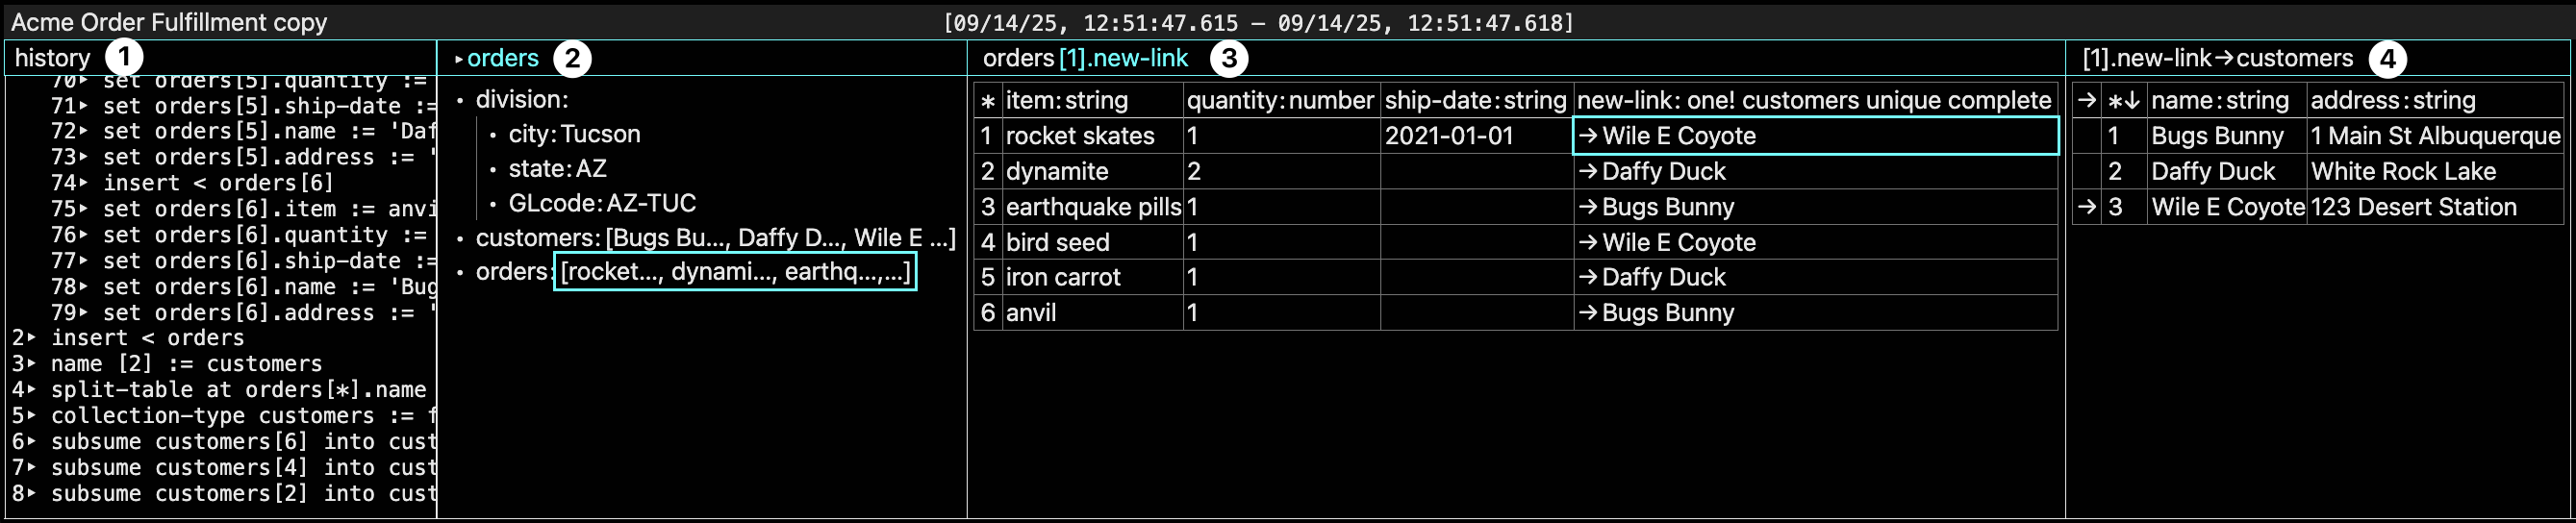
\includegraphics[width=\textwidth]{GUInumbered.png}
\caption{A selection is a path through Miller columns containing indented outlines and flat tables.}
\label{fig:UI}
\end{figure}

\circledtextset{resize=real, charf=\LARGE\sffamily}

The following discussion concentrates on the rationale behind the key UI design decisions.
Figure~\ref{fig:UI} displays a screen shot. \circledtext{1} The left hand column shows the history of operations on this database. History sidebars are a common technique but we were particularly inspired by Wrangler~\cite{kandel11}.

The three columns to the right are Miller columns~\cite{miller-columns} that display a path drilling into and across nested data structures. Usually Miller columns display a simple list, as in the MacOS Finder column view of directories. We elaborate that convention to show in each column either an indented outline or a flat table. Nested structures are indicated with summaries that when clicked open a new column to the right. Cyan outlines show the selected path through the columns. \circledtext{2} is the top-level structure of this document. \circledtext{3} is the \textsf{orders} table within it. The user has selected a link to the \textsf{customers} table, which is opened in the column \circledtext{4}. Selection not only drills into nested structures but also follows links crossing the hierarchy, as if the target table of the link was nested inside it. This design was inspired as a reaction to Ultorg~\cite{bakke:phdthesis, ultorg} which uses nested tables to represent queries crossing a flat relational database. Ultorg provides a single view of a nested structure whereas our use of Miller columns provides only a view of the context of a path within the structure. The compensation for that restriction is that each column contains a visually simpler and context-independent layout, keeping neighbors at each level adjacent to each other rather than being splayed across lower layers.

\begin{figure}[h]
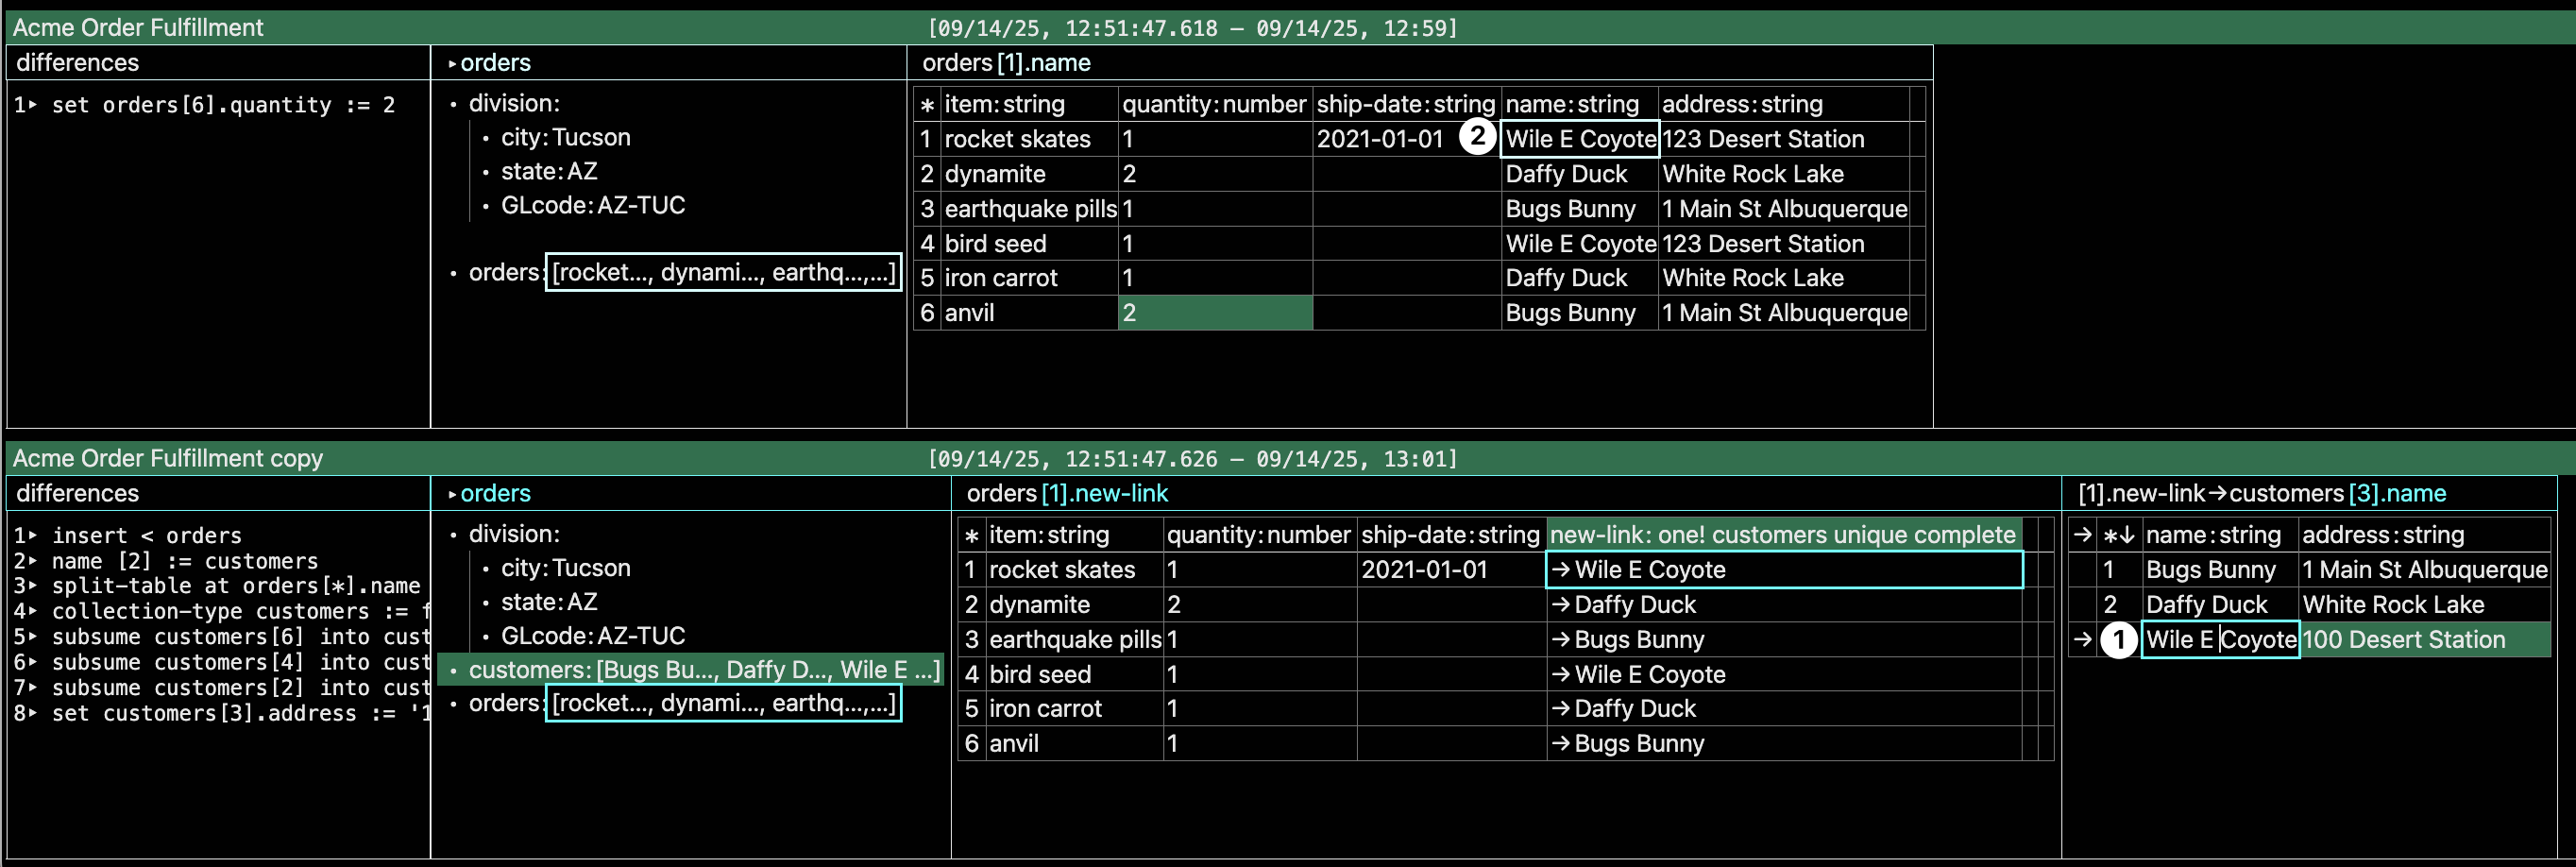
\includegraphics[width=\textwidth]{DiffNumbered.png}
\caption{A diff is displayed across a split screen with coordinated selection.}
\label{fig:Diff}
\end{figure}

Figure~\ref{fig:Diff} displays our representation of diffs. The challenge is that Operational Differencing can do fine-grained comparisons across schema changes. We split the screen in half vertically to compare two databases. Here we are displaying the differences due to database normalization between Figure~\ref{fig:tables-single} in the top half and Figure~\ref{fig:tables-dedup} in the bottom half. Differences on each side are given a green background, and the context menu on them provides a command to transfer that difference to the other side.

The hard problem is not showing what has \textit{changed} but showing what is the \textit{same} across complex structural transformations.
We use \textit{coordinated selection}:  At \circledtext{1} the cyan outline indicates we have selected the \textsf{customers} table cell containing \textsf{Wile E Coyote}. At \circledtext{2} the corresponding cell in the other database has been outlined in white, even though it is in the \textsf{orders} table. We automatically compute the corresponding location of the selection by transfering a \textsf{noop} operation to the other side.

We first tried conventional representations of textual diffs, both side-by-side and interleaved (AKA unified). They have the advantage of keeping corresponding locations close to each other on screen, but only when the differences are limited to inserting and deleting text. They did not adapt well to complex data structures and complex structural transformations. Our split-screen approach handles these cases as well, and has the advantage that the diff view keeps the layout of the data the same as in a normal view.
% However only observation of actual usage will tell how successful this design really is.
% To increase the saliency of coordinated selection we would like to add hover effects and side-by-side ``minimaps'' that use color coding to give a global view of the mapping.



\section{The Playable Demo}\label{demo}

It is difficult to convey the experience of an interactive user interface in a written narrative, so we have developed a \textit{Playable Demo}. We adopt \textit{onboarding} techniques that commercial software uses to teach new users. A scaffold over the UI walks the user through a demo scenario, stepping through a written narrative that prompts each user action. Users that follow the main quest are given a frustration-free experience going at their own pace. The more adventurous are free to roam at their own risk, but can always respawn where they left the path. The demo can be accessed at \url{https://thebaseline.dev/Prog26submission/}. We encourage viewers to share their experience in a survey at the end.

Can a playable demo do a better job explaining new user interface ideas than
written narratives and recorded demos? Our early results are mixed.

\begin{itemize}
\item Using an open source onboarding library was a mistake. A fully integrated experience requires a fully custom implementation.
\item To make a playable demo robust it needs to know exactly what each user step should do and validate it. Specifying that with code is laborious (so much so that we did not do it). Instead we should use the history recorded in a play-through as an oracle. That would also allow ``fast forwarding'' through the demo, a repeated user request.
\item A well-presented demo can lull viewers into suspending disbelief. A playable demo is brutally realistic. Lack of polish is glaringly obvious. Going off script quickly reveals holes in the prototype implementation. These effects make playable demos a risky proposition in competitive academic venues.
\item Despite these negatives, users consistently report that when following the script they feel they understand what is being presented.

\end{itemize}




\section{Technical Dimensions}\label{tech-dims}
% https://tomasp.net/techdims/#footer=index,navigation;left=catalogue,list;top=catalogue,index
We can heuristically evaluate Baseline using the \textit{Technical Dimensions of Programming Systems}~\cite{techdims} framework.
% but we designed the system with these goals in mind

\paragraph{Interaction} Strictly speaking Baseline has two \textbf{modes of interaction}: user and developer, however user mode is a strict subset of developer mode (no type operations) so it is fair to say there is really only one mode of interaction.
Operationalized queries minimize \textbf{abstraction construction} since they correspond exactly to interactive actions in the UI, suporting Programming by Demonstration.
% An intriguing question is how well we can hew to this principle as we add general programming language capabilities following the path previously explored in Subtext~\cite{reifying-programming, direct-programming}.
Operationalizing all change shortens \textbf{feedback loops}: The Gulf of Evaluation is reduced because all operations are concrete direct manipulations; The Gulf of Interpretation is reduced by visualizing changes in terms of concrete difference operations. Version control of data enables collaborative feedback loops that are not practical with conventional techniques.

\paragraph{Notation} Baseline currently has a \textbf{primary notation} that is both a \textbf{surface and internal notation}: sequences of operations. However we expect general programming language features will use a superset \textbf{overlapping notation} that evaluates into the base one. Arguably because Baseline involves a rich set of operations they do not form a \textbf{uniform notation} and generate a complex \textbf{expression geography}.
% In future work we want to investigate whether there is a normal form for sequences of operations.

\paragraph{Conceptual structure} Baseline is attempting to build a common mechanism for all dimensions of change management, in order to maximize \textbf{conceptual integrity} even at the cost of \textbf{openness}. Our approach to \textbf{commonality} rejects the  dichotomy between static/explicit and dynamic/implicit structure: all structure is explicit but can be dynamically refactored as needed. \textbf{Composability} is uniformly through operation sequencing.

\paragraph{Customizability} Operations are executed interactively without \textbf{staging}, but operations cen be staged in branches and transferred later when desired. Baseline is not \textbf{self-sustaining} because it is not implemented in itself and we do not hold that as a goal. Our ID-annotated tree structures provide some level of \textbf{addressing and externalizability}.

\paragraph{Complexity, Errors, and Adoptability} Baseline is still very immature in these dimensions.





\printbibliography

\end{document}

% Local Variables:
% TeX-engine: luatex
% End:
